%% Template for a preprint Letter or Article for submission
%% to the journal Nature.
%% Written by Peter Czoschke, 26 February 2004
%%

\documentclass{nature}
%\documentclass[12pt]{article}

%% make sure you have the nature.cls and naturemag.bst files where
%% LaTeX can find them

\bibliographystyle{naturemag}

\usepackage{graphicx}
\usepackage{amssymb,amsfonts,amsmath}
\usepackage{subfigure}
\usepackage{stfloats}


%% OPTIONAL MACRO DEFINITIONS
\def\s{\sigma}
\newcommand{\be}[0]{\begin{equation}}
\newcommand{\ee}[0]{\end{equation}}
\newcommand{\lb}[0]{\left(}
\newcommand{\rb}[0]{\right)}


\title{Inefficacy of stratospheric sulfate aerosol injections for saving the West Antarctic Ice Sheet}

%% Notice placement of commas and superscripts and use of &
%% in the author list

\author{Kyle C. Armour$^{1}$ \& Gerard H. Roe$^2$}
\author{K. E. McCusker,$^{1}$ \& D. S. Battisti,$^{2}$ \& C. M. Bitz,$^2$}

% NatGeo requirements:
% Title If possible, the title should give a sense of the main new finding, and should not exceed 90 characters, including spaces. Nature Geoscience titles do not contain technical terms or abbreviations unless absolutely necessary. We strongly discourage punctuation or active verbs.@@
% Letter 2,000 words no methods, 3 figures
% Article 3,000 words no methods, include section titles, 6 figures


\begin{document}

\maketitle

\begin{affiliations}
 \item School of Earth and Ocean Sciences, University of Victoria, Victoria, British Columbia, V8V 1B5 Canada
 \item Department of Atmospheric Sciences, University of Washington, Seattle, WA 98195
\end{affiliations}


\begin{abstract}
Solar radiation management (SRM) via injection of sulfate aerosols into the stratosphere has garnered attention for its potential to reduce the climate impacts of global warming, including sea level rise. However, dynamical feedbacks that arise from the combination of stratospheric sulfate aerosols and tropospheric greenhouse gases have not been considered, and may cause nonlinear behavior in subsurface ocean temperatures. Here we investigate in a fully-coupled global climate model (GCM) whether rapidly increasing stratospheric sulfate aerosol concentrations will not only reverse steric sea level rise, but also preserve Antarctic ice sheets, avoiding sea level rise due to mass input. We contrast this SRM method with an idealized scenario in which all greenhouse gases (GHG) are returned to preindustrial levels. We find that the rapid addition of a stratospheric aerosol layer does not effectively counteract upper and surface level atmospheric circulation changes caused by increasing greenhouse gases. Anomalous surface westerlies impose a stress on the Southern Ocean that causes Ekman pumping of relatively warm Circumpolar Deep Water (CDW) to the level of ice shelves. The large-scale oceanic environment under stratospheric sulfate aerosols thus leaves open the possibility of ice sheet destabilization through increased basal melt even in the absence of large atmospheric warming, providing a potentially large source of sea level rise. Meanwhile, removal of atmospheric greenhouse gases restores the wind stress on the ocean, yielding relatively cooler subsurface ocean temperatures. 

\end{abstract}



%\section{Introduction}

Stratospheric sulfate injections may be effective at reducing climate changes due to increased greenhouse gases in that the strategy reduces global averaged temperature and precipitation in many numerical models (e.g., \cite{kravitz13}), although not equivalently \cite{bala08}. Regional disparities also remain \cite{ricke10}, including limited success at eliminating climate change  in the polar regions for a variety of reasons \cite{mccusker12}. Inhomogeneities arise due to differences in the dynamical responses of the atmosphere to forcing by stratospheric aerosols and forcing by increased carbon dioxide \cite{ammann10,mccusker12}. Finally, a single rate of solar radiation management implementation cannot equally avoid changes in components of the climate system with different response timescales, such as surface temperature and sea level rise \cite{irvine12} (because thermosteric sea level rise significantly lags a radiative forcing increase and its associated surface temperature response; e.g., \cite{wigley06,solomon10}). 
%. Deploying a stratospheric sulfate aerosol layer may avoid some of the severe consequences of increased GHGs, especially in the tropics, but the aerosols are not as effective at eliminating climate change in the polar regions for a variety of reasons \citep{mccusker12}. Inhomogeneities arise due to differences in the thermodynamics of the forcings (shortwave versus longwave), differences in the 4-D structure of the forcing within the atmosphere, as well as due to differences in the dynamical response of the atmosphere to these two forcings \citep{ammann10,mccusker12}. Finally, a given rate of solar radiation management implementation cannot equally avoid changes in components of the climate system with different response timescales, such as surface temperature and sea level rise \citep{irvine12}. % Diverse regional temperature and precipitation anomalies remain, but they are generally smaller than regional anomalies due to increasing GHGs without sulfate injections \citep{ricke10}.

%the varying response timescales of different components of the climate system means that SRM cannot equally stabilize global mean surface temperature and sea level rise, for instance \citep{irvine12} @@.  

%Finally, the ability of solar radiation management to curb sea level rise depends critically on the rate at which SRM is implemented; reversing rising global mean sea level requires  

%Finally, the response time of various components of the climate system will yield varying degrees of effectiveness at avoiding %Optimization of unequal changes in climate variables and in climate regions has been carried out@@  % ; a stratospheric sulfate layer is ineffective at reducing atmospheric circulation anomalies due to increased CO$_2$ \citep{mccusker12}

To promptly avoid sea level rise in the face of rising greenhouse gases then, a large and rapid shock of stratospheric aerosols would need to be deployed to stop and reverse heat uptake by the ocean. The amount of aerosols that would be necessary depends on the flux imbalance at the surface (i.e., for how long greenhouse gases (GHGs) accumulate in the atmosphere before initiating climate engineering) and so delayed implementation requires greater solar radiation management (SRM) to immediately counter rising sea levels. Moreover, delayed implementation would yield additional deep ocean heat storage, which may linger at intermediate depths indefinitely \cite{gillett11}. Thermal expansion is not the only mechanism by which sea level can change, however. Ocean volume is modified by density changes due to changes in temperature and salinity, and due to mass inputs including ice sheet melt. Observed sea level rise in recent decades is attributed primarily to thermal expansion, however contributions from runoff and ice sheet melt are expected to grow in the future as surface and ocean warming continue \cite{bindoff07}. 

%: contributions include changes in precipitation, evaporation, freshwater runoff, and ice sheet melt. Observed sea level rise in recent decades is attributed primarily to thermal expansion (thermosteric sea level rise), however contributions from runoff and ice sheet melt are expected to grow in the future as surface and ocean warming continue \citep{bindoff07}. 
 
%[@@REMOVE/REDUCE] The disparate timescales inherent to the climate system response to radiative forcing introduce other inhomogeneities, the most obvious being the fast response of land surfaces versus the `recalcitrant' response of the deep ocean \citep{held10}. Solar radiation management (SRM) of any kind will introduce trade-offs between, for example, the rate at which land is cooled and the rate of sea level change due to thermal expansion \citep{irvine12} - the latter significantly lags the radiative forcing and surface temperature response (e.g., \cite{wigley06,solomon10}). The range of timescales associated with the regional response to forcing has important implications for SRM strategies attempting to avoid climate changes due to GHG increase. For example, should the goal of SRM be to cool the land surface temperature and thus reduce the climate stress on ecosystems and grain yields, the rate of temperature change imposed by SRM may need to be slow, e.g., within the range of trends over the last century. In contrast, to promptly avoid thermosteric sea level rise, the goal of SRM would be to stop and reverse heat uptake by the ocean. In the case of sulfate injections, a large and rapid shock of stratospheric aerosols would need to be deployed to accomplish that goal. The amount of aerosols necessary depends on the flux imbalance at the surface (i.e., for how long greenhouse gases accumulate in the atmosphere before beginning climate engineering) and so delayed implementation means stronger SRM would be required to immediately counter rising sea levels. Moreover, delayed implementation would mean additional deep ocean heat storage, which may linger at intermediate depths indefinitely \citep{gillett11}. %more persistent deep ocean change  % which, because of the long timescale of the ocean, requires a larger radiative forcing than what is needed to simply cool surface temperatures
%. Delaying implementation not only means stronger SRM would be required, but more heat   % \citep{mccuskerinprep} %  --- and maintained, else risking extreme temperature rise (e.g. \cite{mccusker13}) --- 

%[@@ transition from last sentence of first para to this]
%Yet, thermal expansion is not the only mechanism by which sea level can change, however. Ocean volume is modified by density changes (``steric") due to changes in temperature (``thermosteric") and salinity (``halosteric"), and due to mass inputs: contributions include changes in precipitation, evaporation, freshwater runoff, and ice sheet melt. Observed sea level rise in recent decades is attributed primarily to thermal expansion (thermosteric sea level rise), however contributions from runoff and ice sheet melt are expected to grow in the future as surface and ocean warming continue \citep{bindoff07}. 

Curbing sea level rise via SRM has been explored using observed relationships between the response of sea level to volcanic eruptions \cite{moore10}, which have been observed to transiently lower sea level \cite{church05,gleckler06}, and by examining the steric height changes in an intermediate complexity climate model \cite{irvine12}; \cite{irvine12} additionally include the contribution to sea level from mass input with a scaling to the global mean surface temperature anomaly. These studies find that SRM, including with stratospheric aerosol injection, would reduce the rate of global mean sea level rise. However, changes in atmospheric and oceanic circulation, which can have significant impacts on both surface and basal melting of ice sheets and shelves \cite{steig13,joughin11,thoma08}, were not accounted for in the aforementioned studies. The subsurface temperature structure of the Southern Ocean is largely determined by the surface wind stress \cite{fyfe07}, which in turn is set by the circumpolar westerly jet. \cite{mccusker12} showed in a set of idealized simulations that when climate is transiently stabilized using a stratospheric sulfate layer that counteracts growing CO$_2$ concentrations, a residual anomalous poleward-intensified zonal wind stress on the Southern Ocean remains that causes upwelling of warmer subsurface waters to the level of ice sheet outlets. Warmed subsurface ocean waters that destabilize marine ice sheets may introduce nonlinear or threshold behavior \cite{notz09} such that sea level change calculations underestimate the amount of rise for a given surface warming.

%nonlinear or threshold behavior that may arise due to warmed subsurface ocean waters destabilizing marine ice sheets \citep{notz09} is not captured. Changes in atmospheric and oceanic circulation, which can have significant impacts on both surface and basal melting of ice sheets and shelves \citep{steig13,joughin11,thoma08}
%these techniques do not capture nonlinear or threshold behavior that may be introduced by warmed subsurface ocean waters destabilizing marine ice sheets \citep{notz09}.
%however the applicability of these studies to an actual SRM implementation is somewhat limited for different reasons. For example, observationally-based estimates of sea level change assume that climate change during the previous centuries, in which radiative forcing evolved relatively slowly and ocean heat uptake was relatively small, will be applicable in the future after a period of growing radiative imbalance and a vast amount of additional heat absorption by the ocean. Future sea level rise may have a greater proportion of its response that is `in the pipeline' than over the 20th century and this would not be captured by observationally-based estimates of future sea level rise. Likewise, scaling the contribution of mass input to sea level rise with the change in surface temperature assumes there is no threshold behavior. Nonlinearities or thresholds may be introduced by warmed subsurface ocean waters destabilizing marine ice sheets \citep{notz09}. % Additionally, contributions to sea level due to nonlinearities in ice sheet response to ocean warming are not included. 

%Additionally, neither observationally-based nor model-based analyses noted in the previous paragraph address changes in the atmospheric and oceanic circulation, which can have significant impacts on both surface and basal melting of ice sheets and shelves \citep{steig13,joughin11,thoma08}. The subsurface temperature structure of the Southern Ocean is largely determined by the wind stress and the curl of the wind stress \citep{fyfe07}, which in turn is set by the circumpolar westerly jet. Indeed, when climate is stabilized using a stratospheric sulfate layer, anomalous poleward-intensified zonal wind stress in the Southern Ocean remains, and may cause upwelling of warmer subsurface waters to the level of ice sheet outlets \citep{mccusker12}. % \citet{irvine09} modeled the mass balance of Greenland under geoengineering and found that substantial nonlinearities existed based on temperature and precipitation changes, however ocean changes that could affect basal melt of marine outlet glaciers were not considered.  @@
%However, SRM is most likely to be utilized under a scenario in which warming 
 %essentially neglecting the vast amount of heat that the ocean will have absorbed should SRM be necessary; heat that can. 
 %Additionally, dynamical feedbacks are ignored; these may affect the temperature of the water encroaching upon ice sheet outlets. Particularly in the Southern Ocean, atmospheric wind stress changes can substantially influence the subsurface temperature structure \citep{fyfe07}. Indeed, when climate is stabilized using a stratospheric sulfate layer, anomalous poleward-intensified zonal wind stress in the Southern Ocean remains that may cause upwelling of warmer subsurface waters to the level of ice sheet outlets \citep{mccusker12}. @@ more from outline  % Studies have shown that SRM, including stratospheric aerosols, can avoid some amount global mean sea level rise, depending on the rate of implementation \citep{moore10,irvine12}. However, there are multiple 

Realistically, should SRM be utilized, it will likely be after a period of global warming that is deemed to be unacceptably large. Can a rapid implementation of sulfate SRM preserve Antarctic ice sheets and curb potential sea level rise? This question is particularly timely as there are indications that a West Antarctic ice sheet (WAIS) marine instability is already upon us \cite{favier14,rignot14}. Here we investigate the impact of a stratospheric sulfate aerosol layer on the high latitudes of the southern hemisphere (SH), focusing in particular on residual atmospheric circulation changes and associated response in the subsurface ocean. We contrast these results with an idealized scenario in which greenhouses gases are abruptly returned to preindustrial levels --- the ultimate, if not idealized, climate engineering. 

%Thus, does residual atmospheric circulation change, combined with continued ocean heat uptake and associated subsurface warming, leave Antarctic ice sheets in jeopardy? Here we investigate the climate response to a rapid increase of SRM implementation via stratospheric sulfate aerosol injection to determine its effectiveness in the southern hemisphere, particularly to preserve Antarctic ice sheets and curb potential sea level rise. We contrast these results with an idealized scenario in which greenhouses gases are abruptly returned to preindustrial levels. %  (for land ecosystems or ice sheet stability, for instance) % In this chapter, we examine the ability of SRM by stratospheric aerosol injection to avoid sea level rise, and in particular we consider the potential contributions of the ice sheets of Antarctica. 

% other refs: armour et al 2011 (reversibility paper), yin 2011natgeo, stouffer2004?, gillett2011
% @@ what about Moore?
%assumes that contributions to sea level rise by land ice scales with global mean surface temperature.

%fyfe 2007: poleward-intensified winds play a significant role in determining the warming structure of the subsurface southern ocean. wind position primarily determines latitudinal structure and CO2 radiative forcing primarily the amount of warming. sfc wind variations enhance surface warming in the SH beyond that of just CO2. Our simulation is *kind of* like Fyfe's Wind experiment where the winds are that of A2, but CO2 is fixed.
%
%moore 2010: fitting tide gauge obs to different radiative forcings, including volcanic eruptions. one point to make is that the longer the ocean uptakes heat, the more there is available to potentially encroach on Antarctic ice sheets via wind changes. SLR may not be related to observationally reconstructed relationship of SLR and GMT (if I'm understanding their methods at all).

\section{Sea level rise and atmospheric circulation}

The time evolution of global mean surface air temperature (SAT) for business-as-usual (RCP8.5) and climate engineering scenarios is shown in Figure \ref{fig:gmts}a. Sulf (blue) represents a scenario in which drastic climate engineering is required to stop sea levels from further rising, and hence entails a quick and large decrease in net radiative forcing. This decrease in radiative forcing accomplishes a large amount of avoided warming compared to business-as-usual (Figure \ref{fig:gmts}a; RCP8.5 in red). The global and annual mean SAT linear trend for the first decade following the start of SRM (years 2036-2045) is -0.94$^\circ$C/decade for the ensemble mean, and the land-only trend is even greater at -1.2 $^\circ$C/decade. As such, Sulf returns global mean SAT to roughly the end of the 20th century average by the following decade (2045-2054; SAT anomaly of -0.03$^\circ$C) and is much cooler than RCP8.5, which is 1.83$^\circ$C warmer than the end of the 20th century at that time. An instantaneous removal of GHGs to preindustrial conditions (GHGrem in green) is reasonably comparable to Sulf, yielding a slightly overcooled SAT of -0.36$^\circ$C for 2045-2054 compared to the 1970-1999 average. % SFCFLUX here? @@ % ; Table \ref{tbl:means}

Accordingly, global average sea level due to changes in ocean density (representing temperature and salinity changes only) reverses its rising course and starts declining upon initiation of climate engineering (Figure \ref{fig:gmts}b). Nearly 30 cm of sea level rise is avoided by century's end when a sulfate layer is implemented, consistent with previous findings \cite{irvine12}. Thus, assuming no nonlinear or threshold behavior in the contribution of mass input from land ice melt, a high rate of sulfate injection could promptly reduce or avoid sea level rise, at the expense of high SAT trends. %We now turn to the Southern Hemisphere surface and subsurface ocean environment in the context of heat available for melting in ice sheet outlet regions.  % \footnote{Steric sea level change is computed as: $\eta^n = H((\rho_0 / \rho_n) -1)$, where $\eta^n$ is the change in surface elevation at timestep $n$, $H$ is the global mean ocean depth, $\rho_0$ is the `baseline' global mean ocean density from the 20thC simulation averaged over 1970-1999, and $\rho_n$ is global mean density at timestep $n$. Ocean density, $\rho$, is primarily modified by changes in ocean temperature, but is also affected by changes in salinity. This calculation assumes no volume change due to freshwater input (e.g., precipitation, evaporation, river runoff, melting and freezing of sea ice), including neglecting inputs from melting ice sheets, which are not included in the model.}% \citep{mccuskerinprep}
%Quickramp, a goal of which might be to immediately curb sea level rise, does just so and nearly returns steric sea level to 20thC by 2095, at the expense of rapid land SAT trends of almost -1$^\circ$C/decade at the start of SRM.

\begin{figure}%[htbp] % the star afterwards makes it a one column fig in a 2-col document
\centering
 \noindent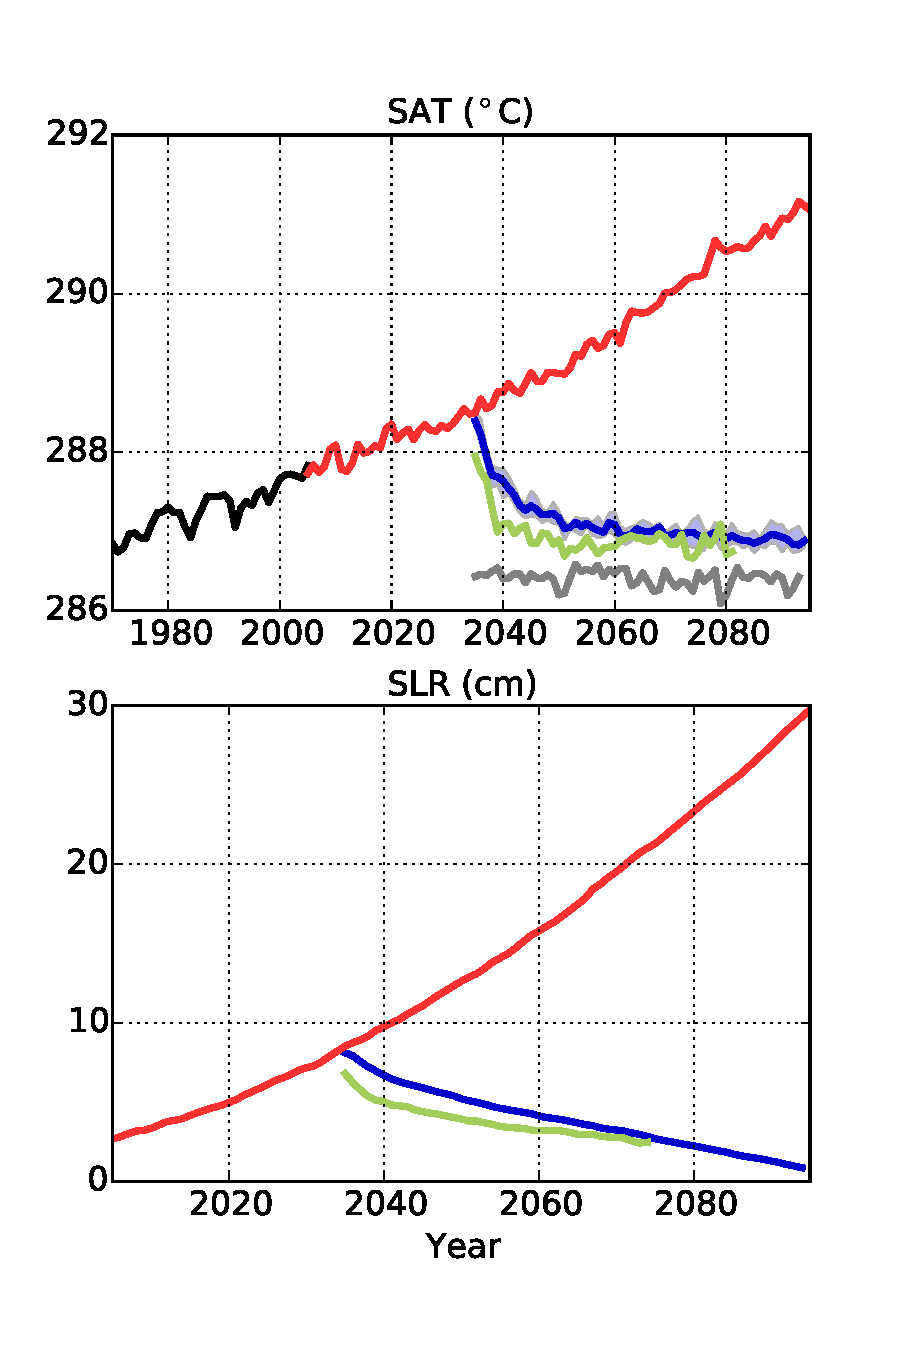
\includegraphics[width=19pc]{figures/SAT_SLR_timeseries_geotimescalesWAISpaper.pdf} %SATSLRtimeseries2.pdf}
\caption{Timeseries of global-mean annual-mean \textbf{(a)} surface air temperature (SAT; $^\circ$C), and \textbf{(b)} steric sea level rise (SLR; cm) due to changes in ocean density, shown as anomalies from 20thC (1970-1999 average). The Sulf curve is an ensemble average. Light blue shading in (a) indicates the spread of the Sulf ensemble of simulations.}
\label{fig:gmts} % @@ do I need to note that years 2076-2078 are interpolated b/c there was missing data?
\end{figure}


%
%
%\begin{figure*}[htbp] % the star afterwards makes it a one column fig in a 2-col document
%\centering
% \noindent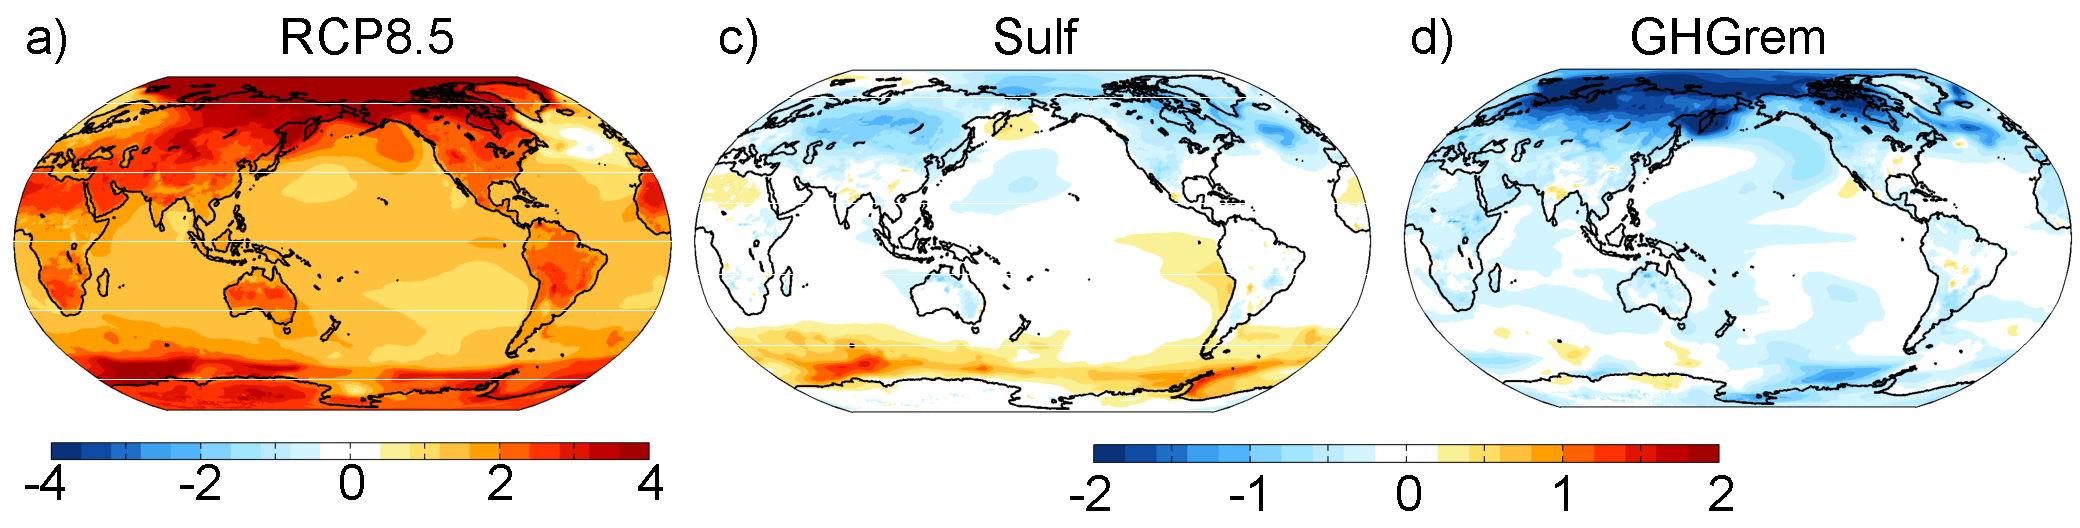
\includegraphics[width=39pc]{figures/SATmaps_noslowramp.pdf}
%\caption{\textbf{Annual mean SAT anomalies.} Annual mean surface air temperature (SAT; $^\circ$C) anomaly from the 20thC (1970-1999 mean) for years 2045-2054 in the following simulations: \textbf{(a)} RCP8.5, \textbf{(b)} Sulf, and \textbf{(c)} GHGrem.}
%\label{fig:satmaps}
%\end{figure*}

%\subsection{Atmospheric circulation anomalies}

Numerical simulations of SRM with stratospheric aerosols have shown residual SH poleward intensified winds induced by differences in the vertical temperature structure of a stratospheric sulfate layer versus well-mixed tropospheric carbon dioxide \cite{ammann10,mccusker12}. These temperature anomalies and corresponding upper atmosphere and surface wind changes share features with those induced by ozone depletion \cite{gillett03,gillett13,sigmond11,thompson11} and increasing greenhouse gases \cite{gillett13,sigmond11,polvani11}. Although mechanisms and structural details differ somewhat depending on the type of upper atmospheric forcing, the fundamental cause is the same: zonal wind shear is modified via thermal wind balance altered by an anomalous increase in the stratospheric pole-to-equator temperature gradient. Strengthened SH lower stratospheric/upper tropospheric winds are then associated with increased eastward eddy propagation, which in turn shifts the critical latitude for Rossby wave breaking poleward, leading to poleward shifted surface westerlies \cite{chen07}.%@@thompson%In the case of stratospheric geoengineering, the vertical zonal mean temperature and zonal wind structure is a confluence of strong tropical lower stratospheric heating due to aerosols and high latitude stratospheric cooling due to GHGs (neglecting the impact of ozone), with little change in the troposphere (cf. Figure 5 from \citet{mccusker12}).  %confluence of a greatly poleward shifted polar vortex due to aerosols with less shifted but greater strengthening due to  
% @@ cite ferraro2011 about strato heating % To some extent, volcanic eruptions also yield similar features (e.g., \citet{free09}), however not significantly in the SH \citep{robock07}, instead being most apparent in NH winter \citep{robock00,shindell04,stenchikov06}.

When aerosols are quickly increased in the stratosphere, large vertical temperature anomalies are generated (Figure \ref{fig:vert}a). The vertical zonal mean temperature structure is a combination of strong tropical lower stratospheric heating due to aerosols \cite{ferraro11} and high latitude stratospheric cooling due to GHGs, with little change in the tropospheric temperature. The resultant zonal winds show a strengthened SH polar vortex and slight weakening of the subtropical jet (Figure \ref{fig:vert}b). %  wherein climate is instead stabilized with a stratospheric sulfate layer, with associated zonal mean zonal wind changes. % ; also compare with Figure 5c from \citet{mccusker12}

\begin{figure}%[htbp] % the star afterwards makes it a one column fig in a 2-col document
\centering
 \noindent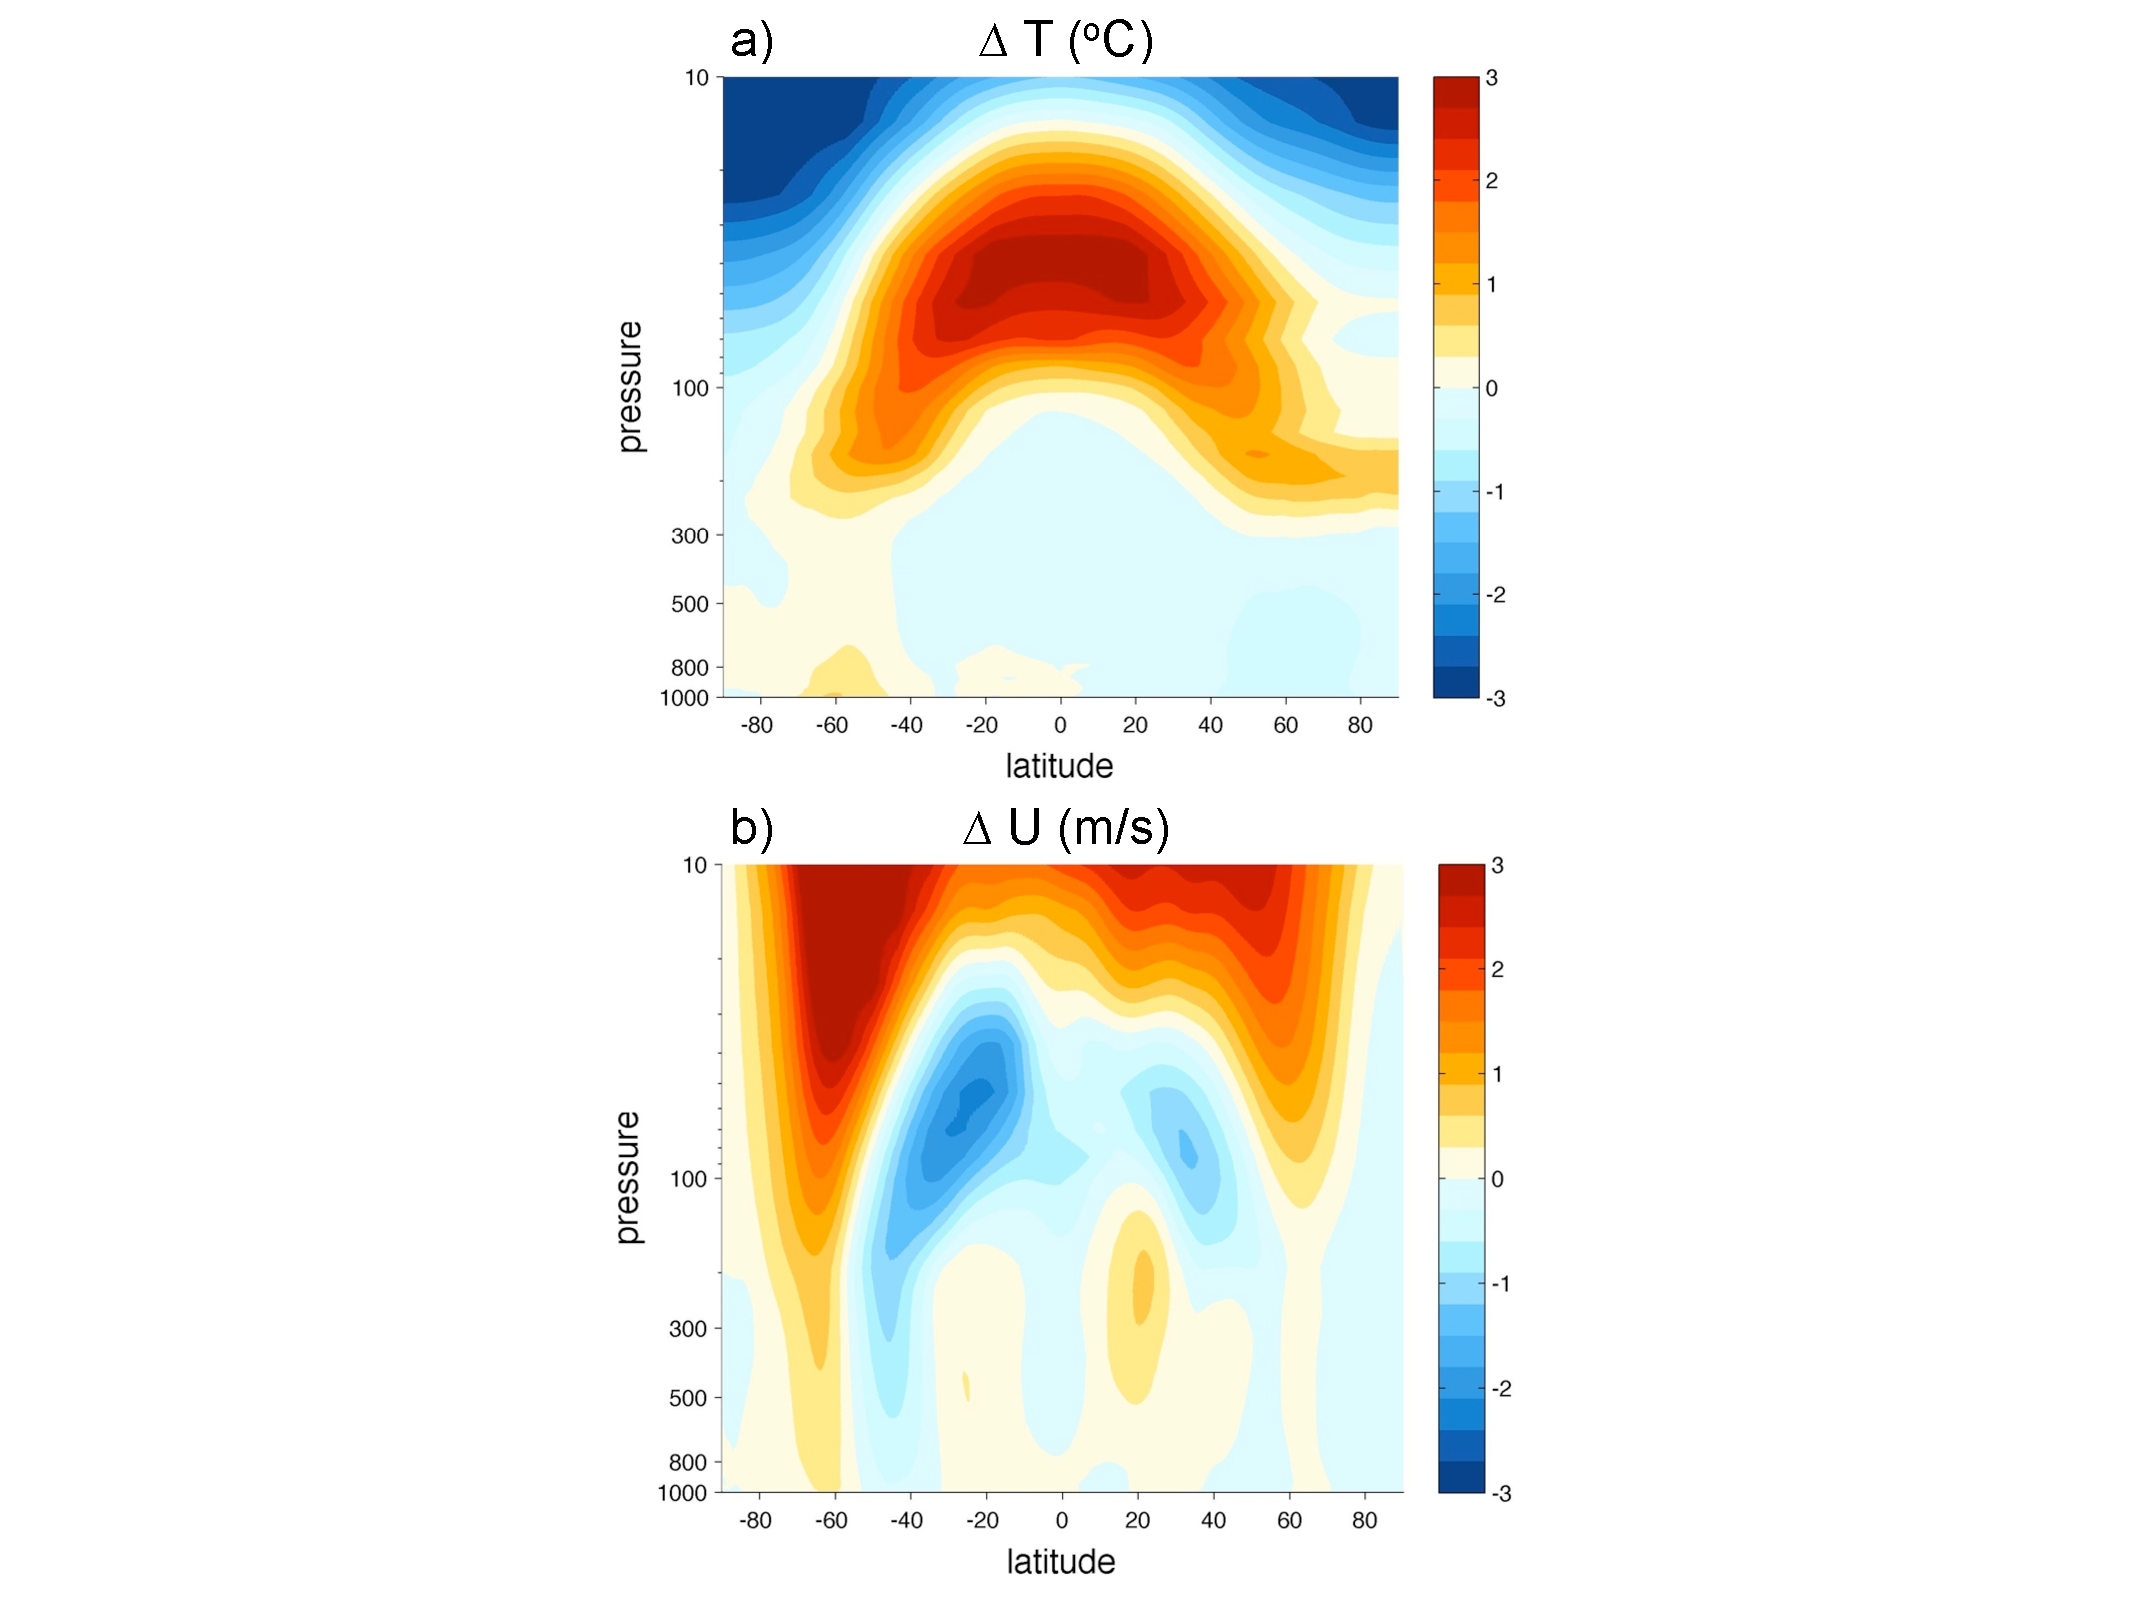
\includegraphics[width=17pc]{figures/verticalU_T_v20thC2.pdf}  % @@  reconfigure to horizontal layout?
\caption{The zonal average \textbf{(a)} temperature ($^\circ$C) and \textbf{(b)} zonal wind (m/s) averaged from 2045-2054 in the Sulf ensemble minus the 1970-1999 average from 20thC.}
\label{fig:vert}
\end{figure}

The upper atmospheric deviations result in surface wind and wind stress anomalies in the SH that are comparable to those in the RCP8.5 business-as-usual scenario: they are poleward-shifted and intensified, and of similar magnitude (Figures \ref{fig:shmaps}d, \ref{fig:shmaps}e, and \ref{fig:zmtautemp}a). In contrast, when GHGs are removed from the atmosphere, the surface wind stress has very nearly returned to 20thC values (Figure \ref{fig:shmaps}f and \ref{fig:zmtautemp}a). Additionally, while both climate engineering strategies cause the sea ice edge to recover to the 20thC position (15\% concentration contours shown in Figure \ref{fig:shmaps}d-f), annual average sea ice concentration near sea ice margins remains lower by up to 15\% in Sulf, but are increased beyond 20thC concentrations by almost 10\% in GHGrem (not shown). The residual sea ice concentration anomalies in Sulf and GHGrem are echoed in the residual temperature anomalies: Figure \ref{fig:shmaps}b shows a small local warming accompanies the reduced sea ice concentration in Sulf, while Figure \ref{fig:shmaps}c shows weak local cooling accompanies the small increase in sea ice concentration in  GHGrem. % This is quite unlike SAT, which is much cooler in Sulf than the business-as-usual scenario (Figures \ref{fig:shmaps}a and \ref{fig:shmaps}b). %(@@consider adding geomip and/or ECHAM here? or appendix?) 
%We note, however, that both climate engineering strategies yield temperature anomalies that are far reduced from the business-as-usual scenario (Figure \ref{fig:shmaps}a).% note that in my CCSM3 results: the aero run has pronounced *decreased* zonal winds over the southern ocean. the stratospheric vortex is strengthened but it's further south than when increased CO2 is also included. 
%Similar vertical temperature anomalies exist when aerosols are quickly increased in the stratosphere in Quickramp (not shown), resulting in zonal mean zonal wind anomalies that rival those in the business-as-usual scenario.  --- that is, poleward intensified zonal mean zonal winds. This is especially evident in the Southern Hemisphere, with a  
%Enhanced surface warming has been associated with poleward intensified winds over the Southern Ocean through increased heat flux from the ocean to the atmosphere via sea ice thickness and concentration changes \citep{fyfe07}. 

\begin{figure*}%[htbp] % the star afterwards makes it a one column fig in a 2-col document
\centering
 \noindent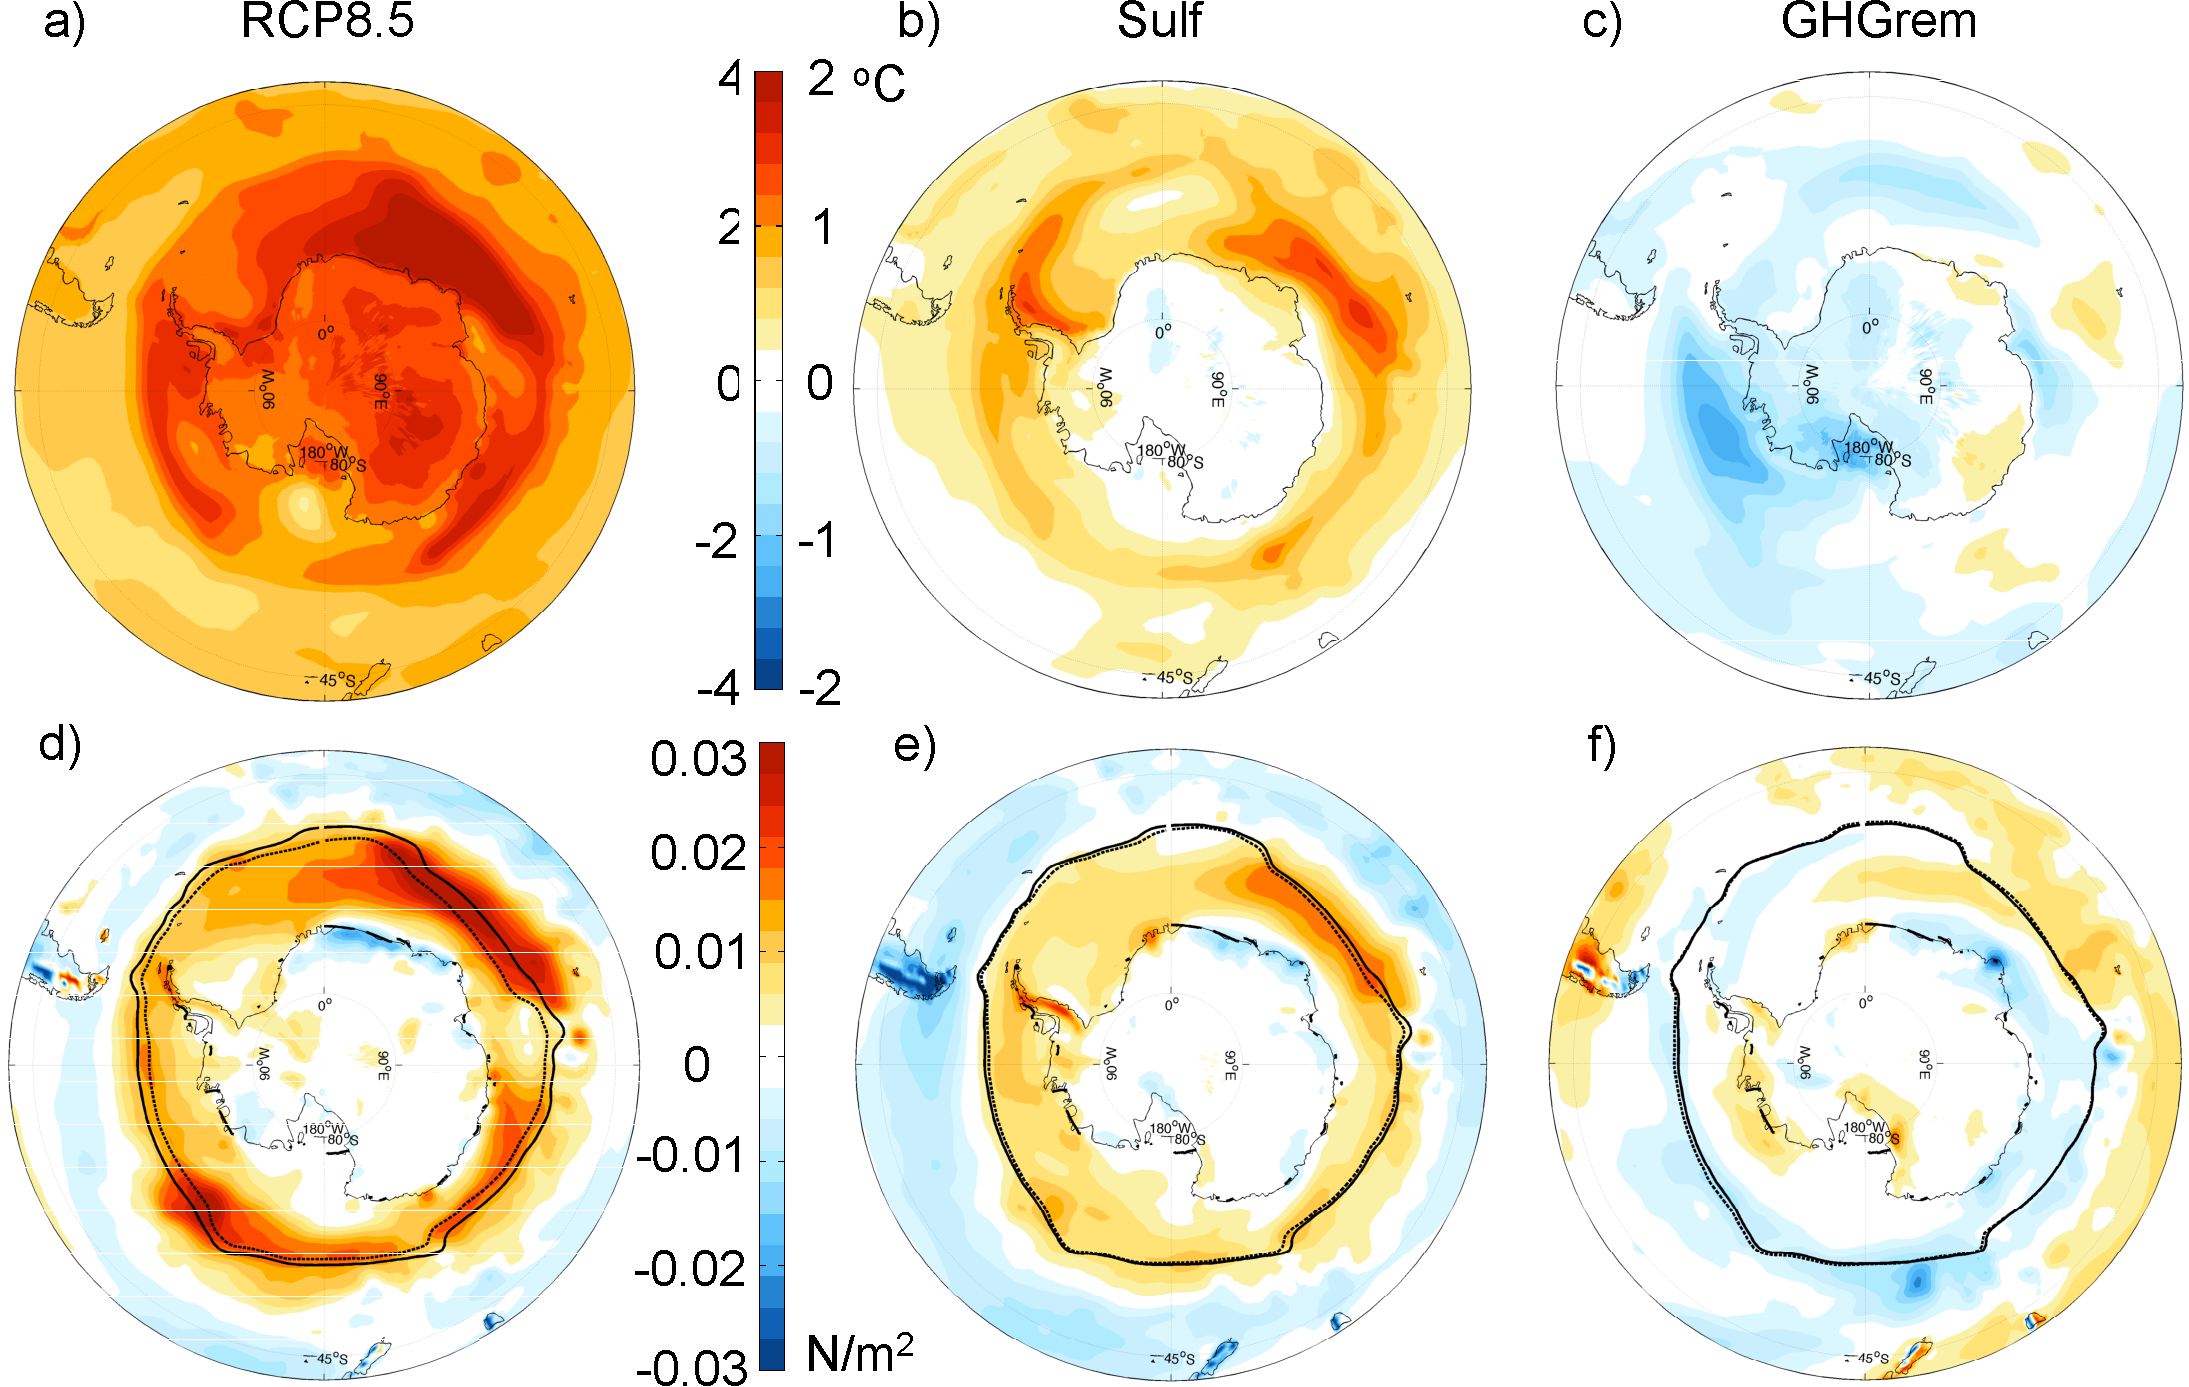
\includegraphics[width=30pc]{figures/SHmaps3.pdf}
\caption{Annual mean surface air temperature ($^\circ$C) anomaly from 20thC (1970-1999 mean) for \textbf{(a)} RCP8.5, \textbf{(b)} Sulf, and \textbf{(c)} GHGrem, years 2045-2054. \textbf{(d), (e), and (f)} are as (a), (b), and (c) but for zonal wind stress (N/m$^2$). Positive indicates westerly stress on the ocean. Contours indicate sea ice extent (15\% concentration contour) for the 20thC (solid) and perturbed simulation (dashed).}
\label{fig:shmaps}
\end{figure*}

%\begin{figure*}[htbp] % the star afterwards makes it a one column fig in a 2-col document
%\centering
% \noindent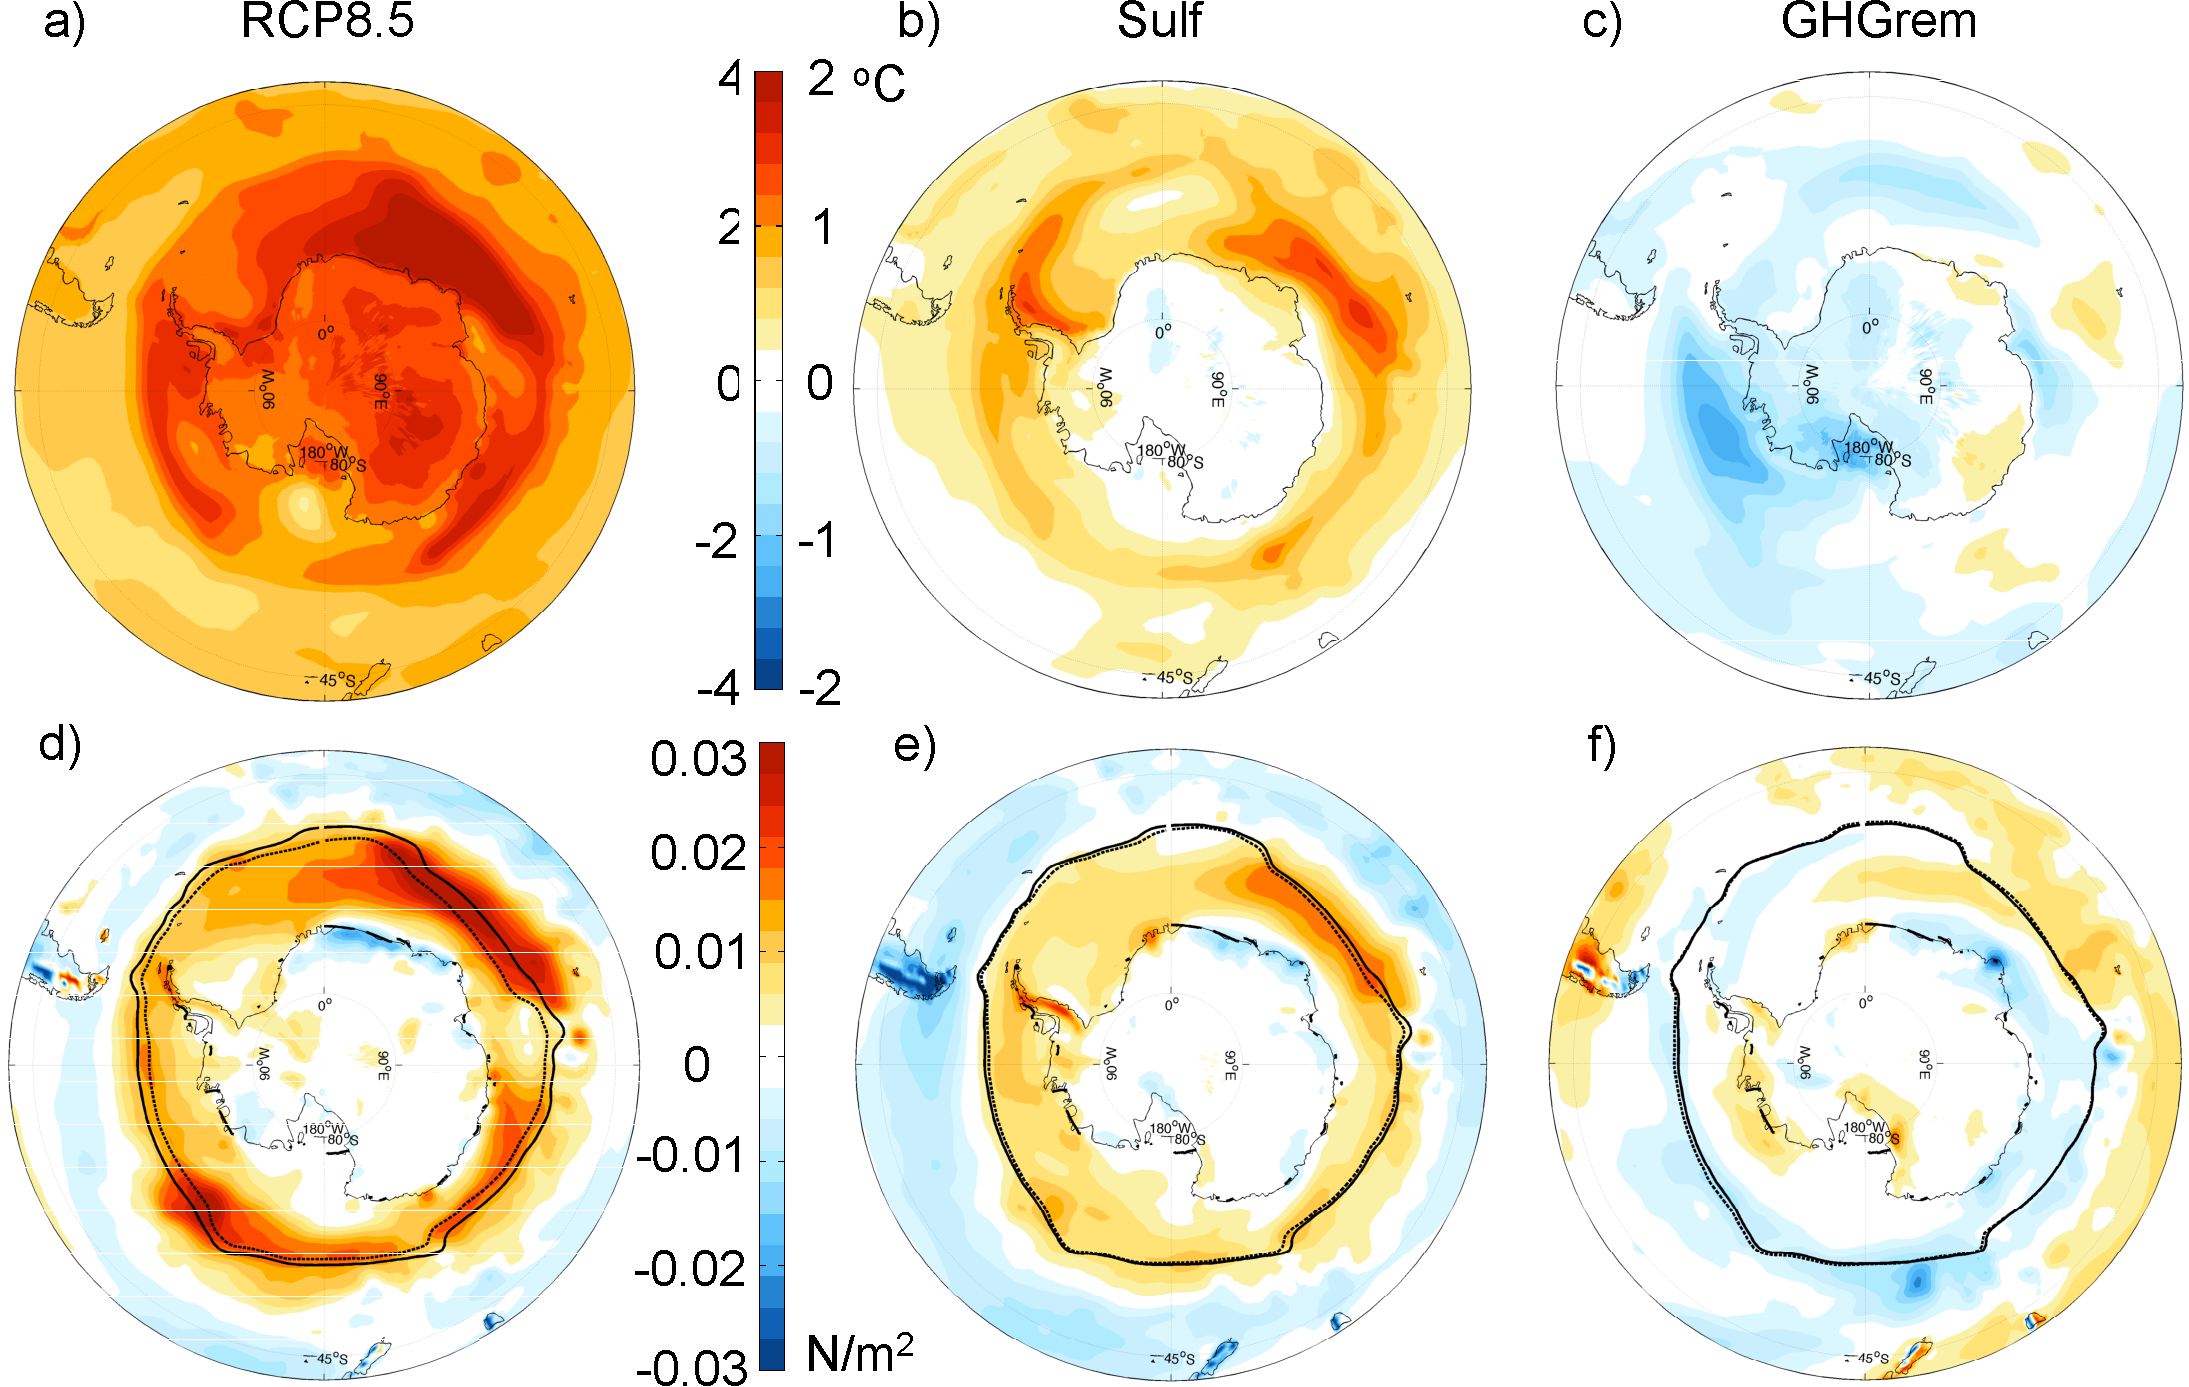
\includegraphics[width=30pc]{figures/SHmaps3.pdf}
%\caption{\textbf{Southern Hemisphere SAT and wind stress anomalies.} Annual mean surface air temperature ($^\circ$C) anomaly from the 20thC (1970-1999 mean) for \textbf{(a)} RCP8.5, \textbf{(b)} Sulf, and \textbf{(c)} GHGrem, years 2045-2054. \textbf{(d), (e), and (f)} are as (a), (b), and (c) but for zonal wind stress (N/m$^2$). Positive indicates westerly stress on the ocean. Contours indicate sea ice extent (15\% concentration contour) for the 20thC (solid) and perturbed simulation (dashed).}
%\label{fig:shmaps}
%\end{figure*}

%\subsection{Implications for Antarctic ice sheets}
%We have seen thus far that rapid sulfate loading and removal of greenhouse gases successfully limit steric sea level rise (Figure \ref{fig:gmts}b), but a key question remains: Given the relatively large circulation and SAT anomalies lingering over the Southern Ocean in Sulf, would sea level contributions from melting ice sheets remain a threat?
%to cool the globe is less effective at cooling the surface and recovering sea ice in the Southern Hemisphere than in the Northern Hemisphere, but that this is not the case when greenhouse gases are removed (at the expense of greater northern high latitude cooling). Our original motivation for simulating such a rapid climate engineering scenario was to investigate whether imminent and potentially dangerous levels of sea level rise could be avoided, even at the cost of large land surface temperature trends. Indeed, each of these strategies successfully limits steric sea level rise (Figure \ref{fig:gmts}b) but a key question remains: Given the relatively large circulation and Southern Ocean temperature anomalies lingering in Sulf, would sea level contributions from melting ice sheets remain a threat? %ice sheet instability or collapse leading to large sea level rise be avoided as well?

\section{Implications for Antarctic ice sheets}
% @@ notes 9/2/2014: Global mean temp for Sulf and GHGrem are similar by year 2060. Comparing the zonal mean TEMP anomalies with depth in year 2060, Sulf shows minor cooling in the surface layer in SO whereas GHGrem has cooling down to greater than 500m. Additionally global mean TOA and OSHF are comparable in the two runs almost immediately (within 5 years) -- implying that the global mean forcings in the two run are comparable right away. However, the southern hemisphere (southern ocean & SH SAT) in the two runs shows very different evolutions. @@calculate a TEMP trend in a SO box in the two runs (say, 200m-500m and ~60S-77S). Add time series of SO or SH SAT to Fig 1?
A large amount of mass loss from ice sheets occurs due to basal melt of their ice shelves \cite{joughin11}, the floating extensions of land ice sheets. In West Antarctica, the face of these ice shelves extend from the surface to several hundred meters depth, near the level of the Circumpolar Deep Water (CDW). The CDW is a subsurface water mass that is slightly warmer than waters above and below it (-1$^\circ$C to 1$^\circ$C; \cite{yin11}). An increase in the temperature of CDW or an increase in the rate that CDW is brought onto the continental shelf due to regional wind variability can greatly increase basal melting of ice shelves \cite{thoma08,joughin11}, causing ice shelf thinning and a subsequent reduction in the buttressing stress, leading to an increase in ice stream velocity \cite{oppenheimer98}. In short, a small warming of CDW, or a greater propensity for it to encroach on continental shelves, has the potential to cause ice shelf disintegration even in the absence of large atmospheric warming \cite{oppenheimer98}. %, in addition to calving and surface melt

Both climate engineering scenarios presented here in Sulf and GHGrem greatly reduce the surface warming in Antarctica that is seen in the RCP8.5 scenario --- over 100\% in the case of GHGrem (compare Figure \ref{fig:shmaps}b and \ref{fig:shmaps}c with \ref{fig:shmaps}a) --- but the significant amount of ocean heat uptake that occurred over the first third of the 21st century before climate engineering was initiated (not shown) also poses a threat to Antarctic ice sheets, particularly the WAIS, whose grounding line is below sea level \cite{joughin11} and retreating \cite{rignot14}. %We thus turn to the temperature structure below the ocean's surface in the vicinity of the Antarctic coast.  % Figure \ref{fig:energyts}b

%\begin{figure*}[htbp] % the star afterwards makes it a one column fig in a 2-col document
%\centering
% \noindent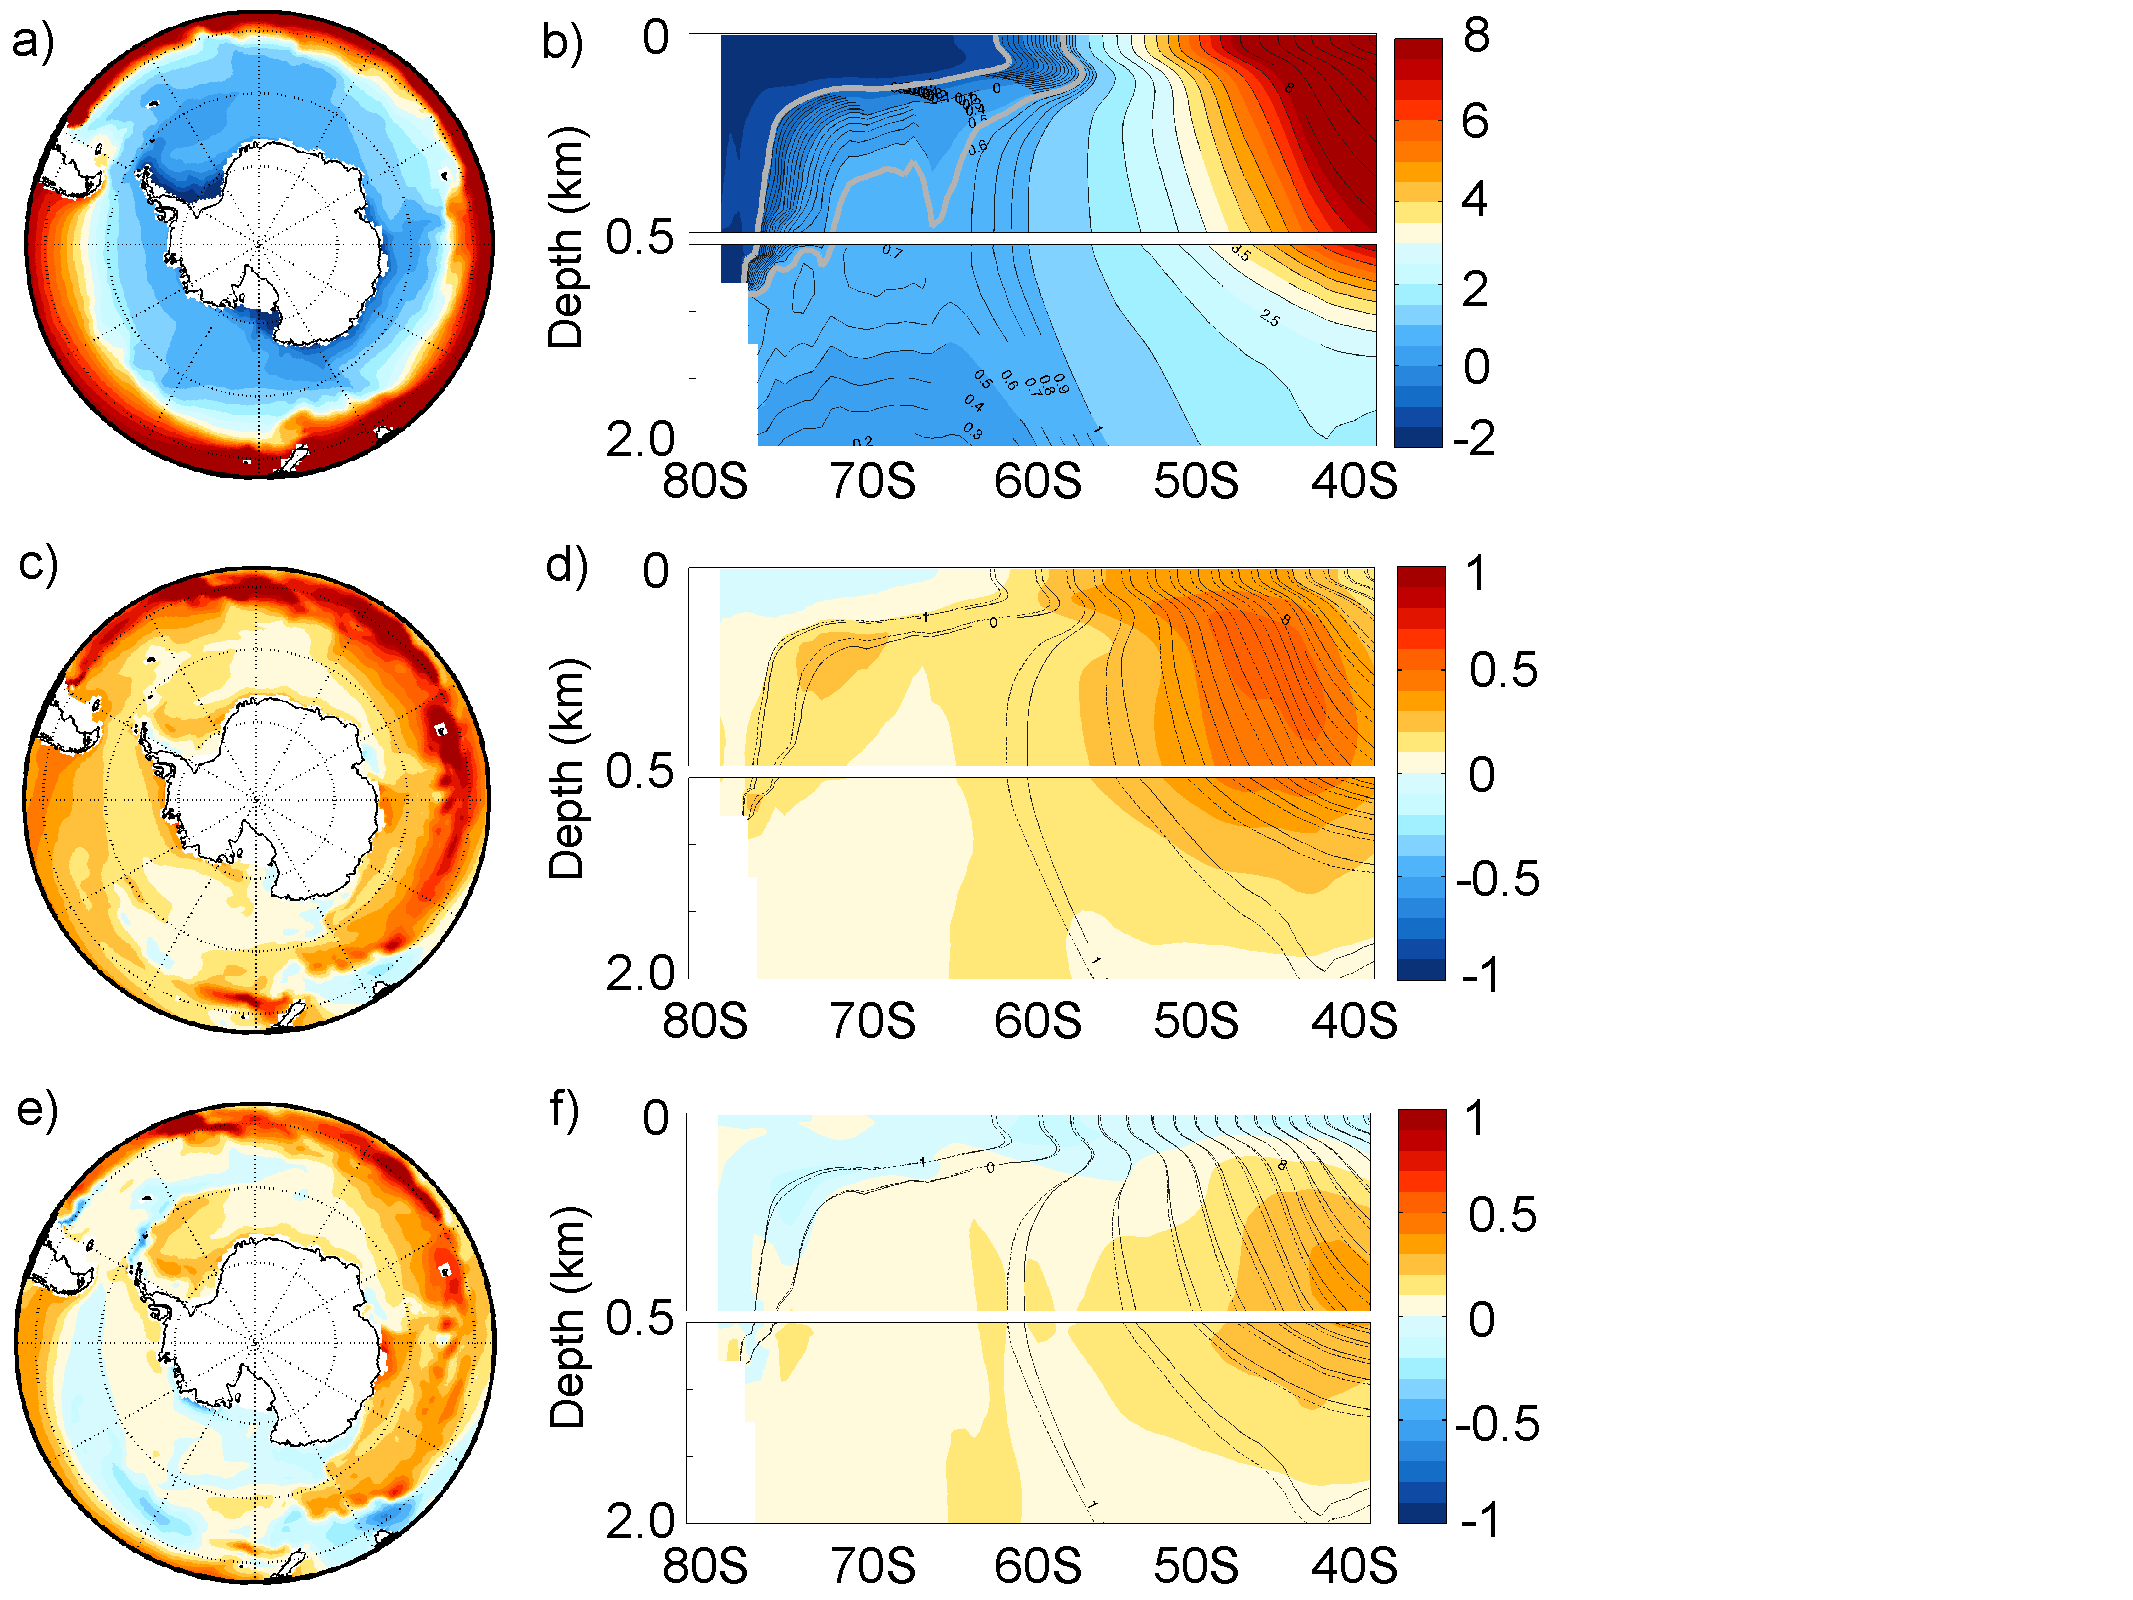
\includegraphics[width=39pc]{figures/SHsubsfcTEMP_wclimo2.pdf}
%\caption{\textbf{Subsurface ocean temperature climatology and anomalies.} Annual mean ocean potential temperature ($^\circ$C) in color, averaged over 200-500 meters depth for the \textbf{(a)} 20thC climatology (1970-1999 mean), and anomalies from climatology in \textbf{(c)} Sulf, and \textbf{(e)} GHGrem for years 2045-2054 in color. Shading in \textbf{(b), (d), and (f)} are as (a), (c), and (e) but show annual mean, zonal mean ocean potential temperature ($^\circ$C) with depth (km). Solid black contours show the 20thC climatology isotherms. Contour interval in (b) is 0.1 from -1$^\circ$C to 1$^\circ$C and 1 for 1$^\circ$C and warmer. The thick, gray isotherms in (b) denote the approximate region in which water warms with depth, estimating the location of CDW (the lower isotherm is 0.6$^\circ$C and the upper is -1$^\circ$C). Dashed contours in (d) and (f) are Sulf and GHGrem isotherms, respectively, with contour intervals of 1$^\circ$C.
%} 
%\label{fig:shsubtemp}
%\end{figure*} % @@ remove this figure. Replace with 

%Southern Ocean subsurface temperature for the end of the 20th century, averaged over the 200-500 m layer is shown in Figure \ref{fig:shsubtemp}a. Mean simulated temperatures generally average between about -1$^\circ$C and 1$^\circ$C along the coastline, slightly higher than the freezing point of seawater (-1.8$^\circ$C). 

Small ocean temperature perturbations can have a significant impact on basal melting of ice shelves; a warming of just 0.1$^\circ$C can thin 1 m of ice shelf in a year \cite{rignot02}. Zonally averaged Southern Ocean temperature anomalies in Sulf indicate that temperatures encroaching on the ice shelves average 0.15-0.20$^\circ$C warmer than 20thC (Figure \ref{fig:zmtautemp}c), which is already a few tenths of a degree warmer than simulated preindustrial conditions (not shown). Drastic reduction of greenhouse gases, however, show zonal mean temperature near the level of ice shelves is up to 0.25$^\circ$C cooler than in Sulf (Figure \ref{fig:zmtautemp}d). Were all of this average extra heat in Sulf to go into basal melt, reducing GHGs rather than deploying stratospheric aerosols would result in 2.5 meters of ``preserved" ice shelf thickness each year. 

%Utilizing stratospheric aerosols to curb global temperatures yields residual ocean warming in the 200-500m layer equal to 0.2-0.3$^\circ$C in many Antarctic coastal locations (not shown). 
%The zonal average Southern Ocean temperature (Figure \ref{fig:shsubtemp}d) indicates that temperatures encroaching on the ice shelves average a few tenths of a degree warmer than 20thC (which is already a few tenths of a degree warmer than simulated preindustrial conditions; not shown). 
%Drastic reduction of greenhouse gases, however, exhibits smaller residual subsurface warming, particularly near west Antarctica (with the exception of the Weddell Sea, which has similar residual warming in the two scenarios; Figure \ref{fig:shsubtemp}e). Average zonal temperature near the level of ice shelves is 0.25$^\circ$C cooler in the reduced GHG simulation than in Sulf (Figure \ref{fig:shsubtemp}f). Were all of this average extra heat in Sulf to go into basal melt, reducing GHGs rather than deploying stratospheric aerosols would result in 2.5 meters of ``preserved" ice shelf thickness each year. 
The anomalous mid-depth warmth evident south of about 65$^\circ$S and between 200-400m depth in Sulf (Figure \ref{fig:zmtautemp}c) can be understood as anomalous upwelling of relatively warm CDW. This upwelling is caused by increased Ekman pumping that originates from the previously discussed poleward-intensified zonal winds (Figures \ref{fig:shmaps}e) caused by stratospheric aerosols, greenhouse gases \cite{fyfe07}, and their combination here (Figure \ref{fig:zmtautemp}a). Sulfate engineering exhibits a more contracted and slightly weaker region of westerly stress anomaly compared to if no geoengineering were applied (RCP8.5), and exhibits greater easterly stress than RCP8.5 equatorward of about 55$^\circ$S (Figure \ref{fig:zmtautemp}a). The curl of the wind stress shows the regions of anomalous upwelling and downwelling in RCP8.5 are retained in Sulf (Figure \ref{fig:zmtautemp}b). %@@rework this and next 2 para

The mid-depth residual warming resembles the 'slow timescale' response to an increase in ozone forcing described in \cite{ferreira14}, wherein Southern Ocean circulation adjusts to changes in atmospheric winds and causes ocean warming from below that overcomes initial SST cooling and sea ice growth on the time scale of decades. Thus, engineering by sulfate aerosols features anomalous upwelling (downwelling) poleward (equatorward) of 60$^\circ$S -- just as in the RCP8.5 scenario (albeit with slightly smaller upwelling than in RCP8.5). In contrast, the removal of GHGs causes a reversal of sign in the zonal wind stress and wind stress curl anomalies compared to the anomalies associated with RCP8.5, resulting in weak anomalous downwelling south of 60$^\circ$S (Figure \ref{fig:zmtautemp}b), which results in the cooling of the 200-400m layer past the 20th century mean (Figure \ref{fig:zmtautemp}d). % and no anomalous warming south of 75$^\circ$S near ice shelves (Figure \ref{fig:zmtautemp}d). The removal of GHGs causes the

Although not germane to the stability of Antarctic ice sheets, it is interesting to note the disparate temperature profiles equatorward of 60$^\circ$S between Sulf and GHGrem as well. The warming evident equatorward of 60$^\circ$S at all depths in Sulf is a combination of residual warmth from pre-geoengineering, a poleward shift (fundamentally due to the atmospheric jet shift) of the nearly vertical isotherms there, and increased downwelling of warmer surface waters. This feature is noticeably absent when GHGs are instead removed from the atmosphere because the jet rapidly returns to the 20thC position, resulting in weak upwelling anomalies equatorward of 60$^\circ$S. Thus the warming equatorward of ~60$^\circ$S is also due to the changes in the atmospheric winds due to the net forcing of increased CO$_2$ and sulfate aerosols.

%These characteristics reinforce the importance of atmospheric wind changes on subsurface ocean temperatures.

%This upwelling is due to increased Ekman pumping originating from the previously discussed poleward-intensified zonal winds (Figures \ref{fig:shmaps}e and \ref{fig:zmtautemp}a) caused by stratospheric aerosols, greenhouse gases \citep{fyfe07}, and their combination here (Figure \ref{fig:zmtautemp}a). 
 %The meridional stream function in the region confirms this, consisting of an anomalous clockwise circulation with upwelling south of about 60$^\circ$S and downwelling to the north (Figure \ref{fig:zmtautemp}c; contours). 
%Sulfate engineering exhibits a more contracted and slightly weaker region of westerly stress anomaly compared to if no geoengineering were applied (RCP8.5), but exhibits greater easterly stress than RCP8.5 equatorward of about 55$^\circ$S (Figure \ref{fig:zmtautemp}a). The curl of the wind stress shows the regions of anomalous upwelling and downwelling in RCP8.5 are retained in Sulf (Figure \ref{fig:zmtautemp}b). Engineering by sulfate aerosols features anomalous upwelling (downwelling) poleward (equatorward) of 60$^\circ$S -- just as in the RCP8.5 scenario (albeit with slightly smaller upwelling than in RCP8.5). % and elsewhere in the Southern Ocean (Figure \ref{fig:shsubtemp}f).  %, indicated by shoaling of the isotherms south of 65$^\circ$S (Figure \ref{fig:shsubtemp}d)

%\begin{figure*}[htbp] % the star afterwards makes it a one column fig in a 2-col document
%\centering
% \noindent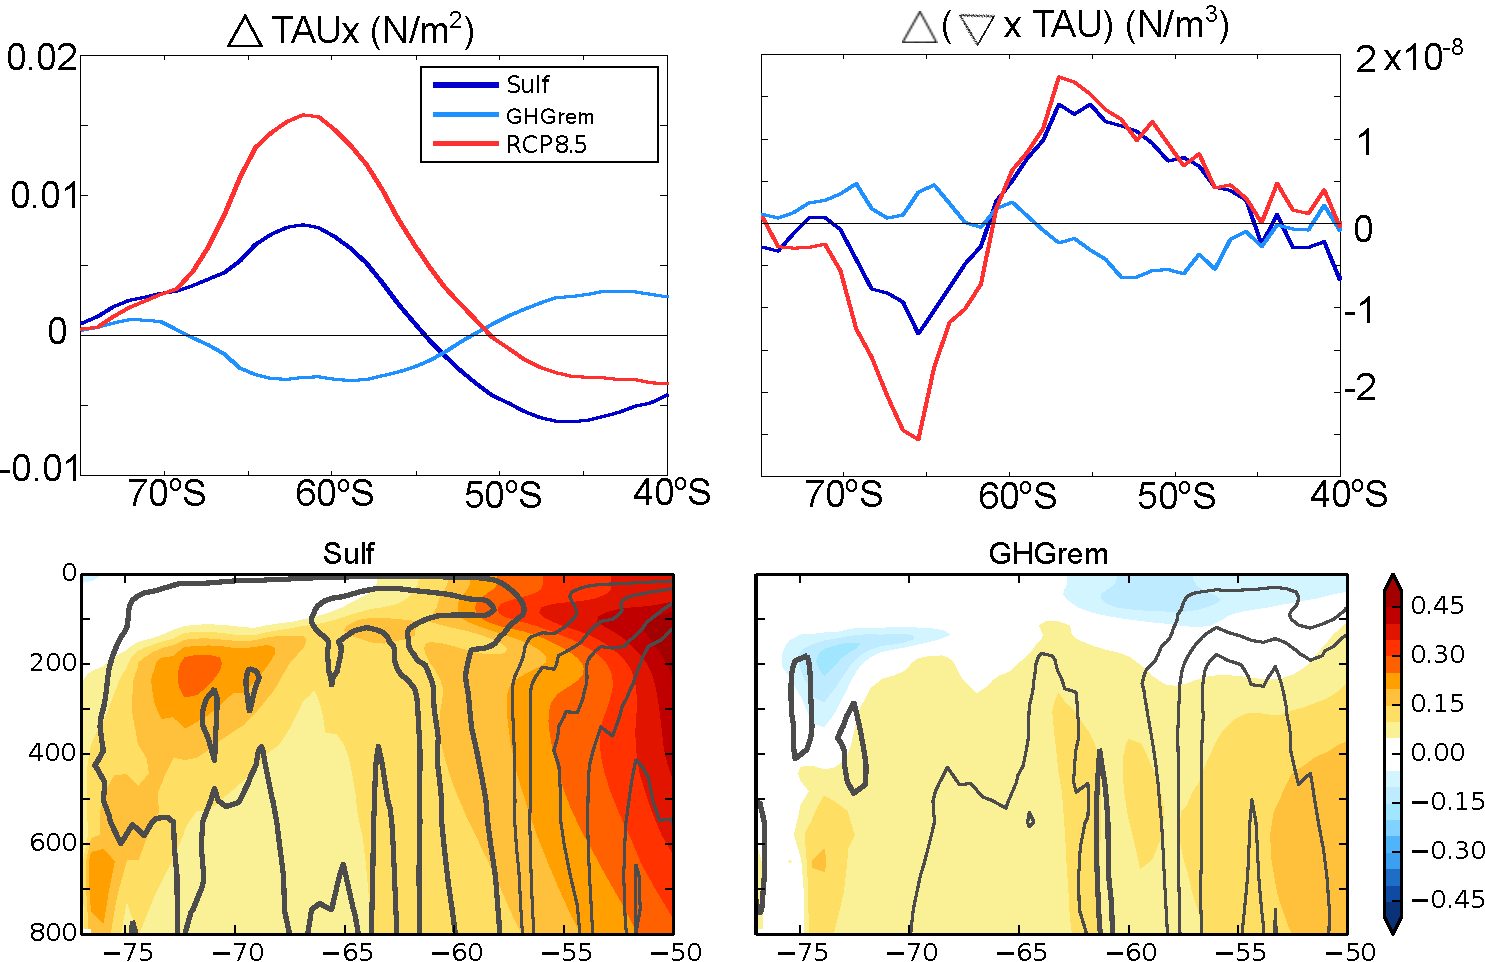
\includegraphics[width=35pc]{figures/TAUcurl_TEMPanomMOCeddy+eul.pdf}
%\caption{Annual mean, zonal mean \textbf{(a)} zonal wind stress (N/m$^2$) and \textbf{(b)} curl of the wind stress (N/m$^3$) over ocean only, as anomalies from 20thC (1970-1999 mean). Positive indicates westerlies in (a) and downwelling in (b). Annual mean, zonal mean ocean potential temperature ($^\circ$C) with depth (shading) and meridional overturning streamfunction (Sv; contours begin at 0.1 with interval 0.5) anomalies from 20thC for \textbf{(c)} Sulf and \textbf{(d)} GHGrem, years 2045-2054. Thick contours indicate positive (clockwise) circulation anomalies and thin contours indicate negative (counter-clockwise) circulation anomalies in (c) and (d).}
%\label{fig:zmtautemp}
%\end{figure*}
\begin{figure*}%[htbp] % the star afterwards makes it a one column fig in a 2-col document
\centering
 \noindent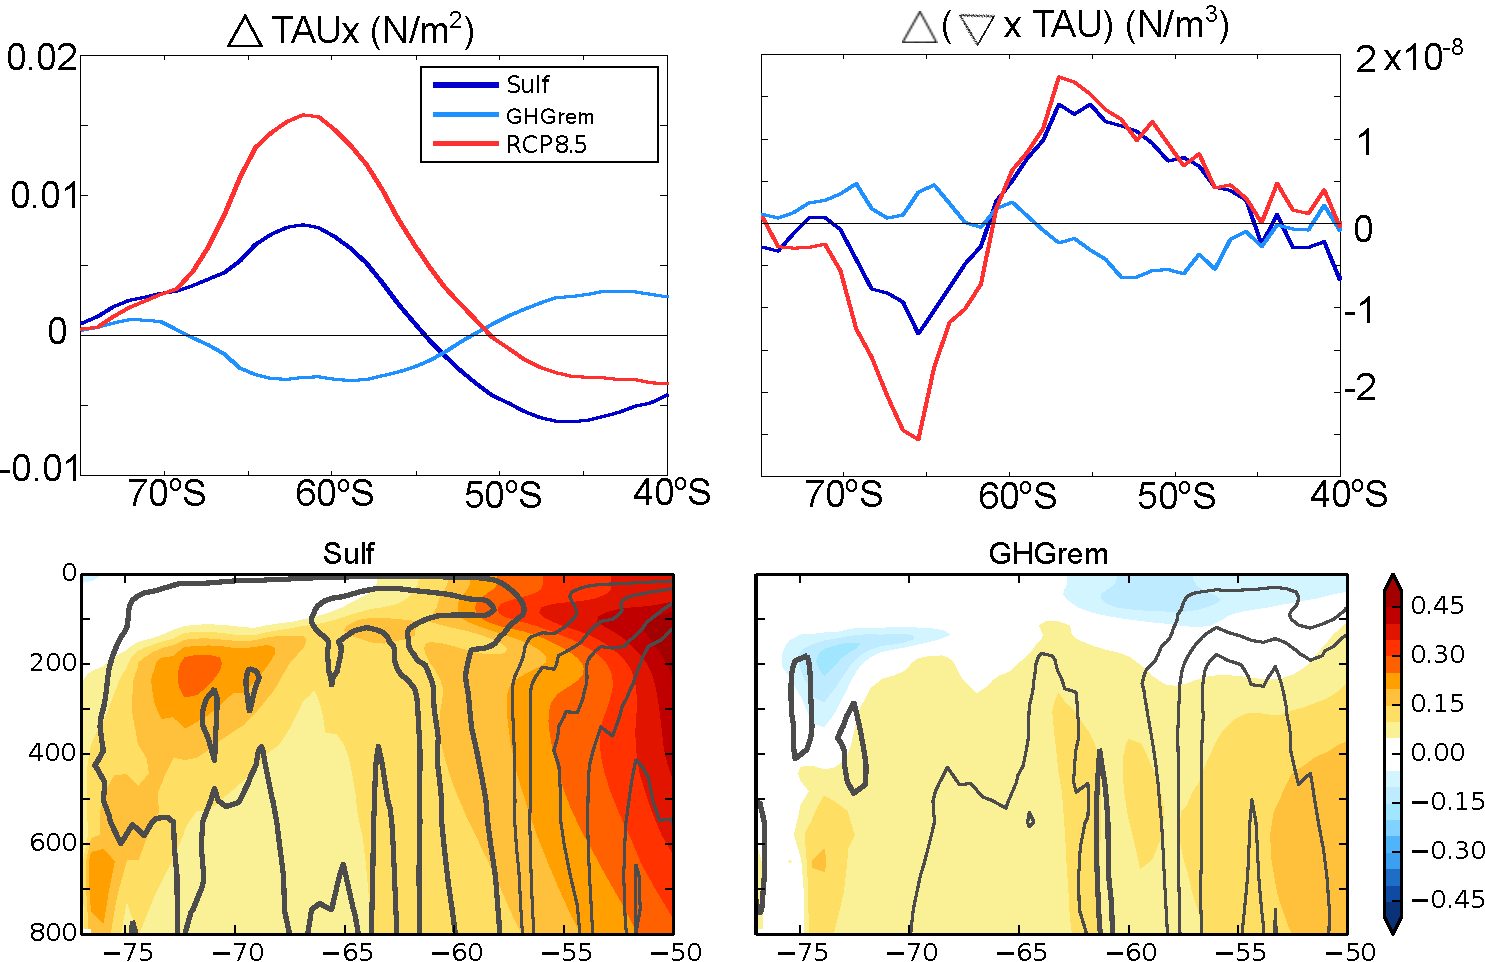
\includegraphics[width=35pc]{figures/TAUcurl_TEMPanomMOCeddy+eul.pdf}
\caption{Annual mean, zonal mean \textbf{(a)} zonal wind stress (N/m$^2$) and \textbf{(b)} curl of the wind stress (10$^{-8}$ N/m$^3$) over ocean only, as anomalies from 20thC (1970-1999 mean). Positive indicates westerlies in (a) and downwelling in (b). Annual mean, zonal mean ocean potential temperature ($^\circ$C) anomalies from 20thC with depth for \textbf{(c)} Sulf and \textbf{(d)} GHGrem, years 2045-2054.}
\label{fig:zmtautemp}
\end{figure*}

These results show that in the zonal mean Southern Ocean, the large-scale oceanic environment remains conducive to basal melting of ice shelves when stratospheric sulfate injections are implemented, but not when GHGs are removed. Examining the most at-risk ice sheet region in Antarctica, the Amundsen Sea Embayment sector including Pine Island Glacier (PIG), reveals an even greater potential for melting under sulfate climate engineering than in the zonal average: the Sulf ensemble features an anomalous residual warming of 0.5$^\circ$C in the 200-500m layer (Figure \ref{fig:pigtemp}a). In contrast, removal of GHGs is effective at cooling the subsurface ocean up to 0.5$^\circ$C, a differential of 1$^\circ$C or 10m of potential ice shelf thickness per year between the two climate engineering methods. Eulerian, eddy, and total components of the vertical advection tendency (in units of $W/m^2$) averaged from 65-74$^\circ$S are shown with depth in Figure \ref{fig:pigtemp}c. There is an increase in temperature due to vertical advection throughout the water column under sulfate engineering (negative values) whereas removal of GHGs causes a decrease (due to the Eulerian component). The primary driver of these disparate tendency profiles is a vertical velocity ($w$) response of opposing signs (Figure \ref{fig:pigtemp}d), primarily Eulerian, acting on a temperature gradient that features an increase in temperature with increasing depth in these layers (Figure \ref{fig:pigtemp}e). %Anomalous temperature equatorward of 65$^\circ$S is explained by the same mechanisms previously described for Figure \ref{fig:zmtautemp}.  %The behavior under sulfate engineering is akin to the 'slow' timescale response to an increase in ozone forcing described in \citet{ferreira14}, wherein warming from below takes years to decades to overcome initial SST cooling and sea ice growth.
%Both scenarios are initiated from a common climate state after the global mean temperature warmed about 1$^\circ$C, and are compared to each other when their global average SAT anomalies are comparable. Atmospheric circulation and hence oceanic circulations respond 
%The primary cause of the contrasting results in the Southern Ocean more broadly, and the PIG region specifically is the disparate response of atmospheric circulation.
%(@@calc Tprime * Wbar for comparison...not as meaningful?)

%Pine Island Glacier is particularly important because it is currently the largest contributor to sea level rise from Antarctica \citep{shepherd12}@@. Moreover, PIG thinning continues to accelerate \citep{rignot08} and may already be in the throes of a marine instability \citep{favier14,rignot14}.

%We conclude by examining the ocean environment in the Pine Island Glacier (PIG) outlet region, where ice shelves have been thinning rapidly \citep{rignot08} and may already be experiencing a marine instability \citep{favier14,rignot14}.@@


\begin{figure*}%[htbp] % the star afterwards makes it a one column fig in a 2-col document
\centering
 \noindent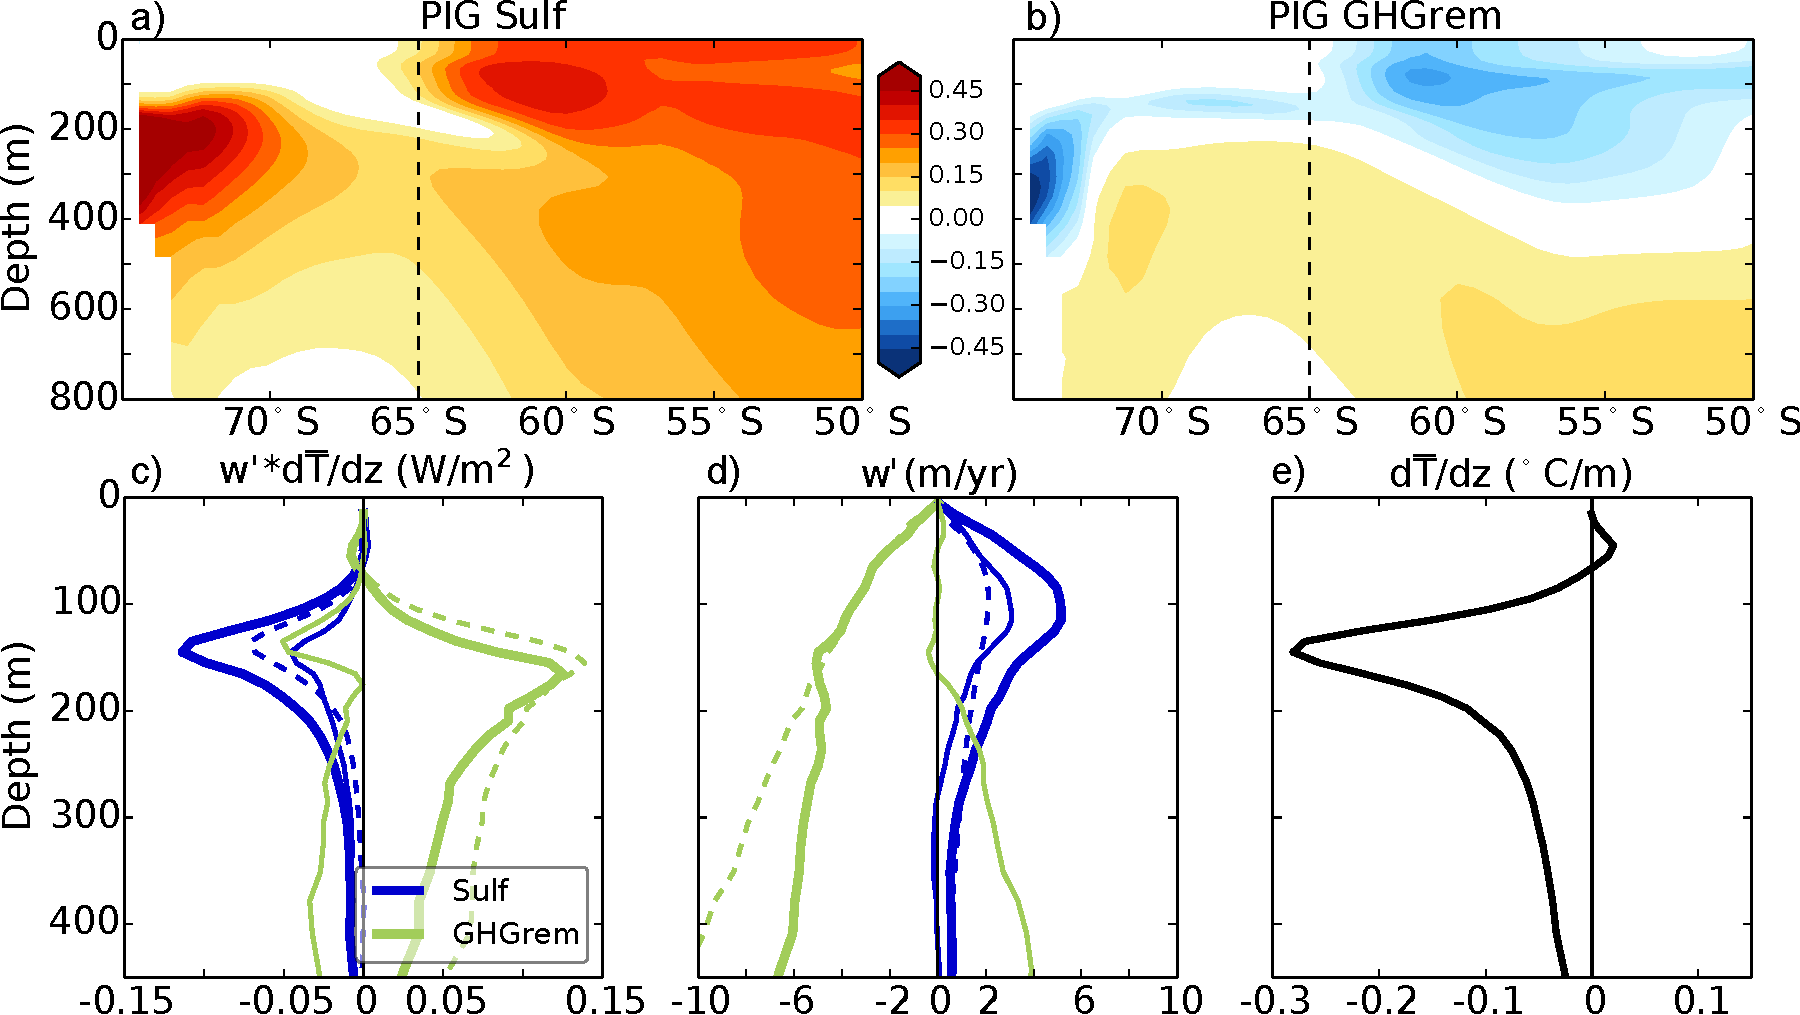
\includegraphics[width=35pc]{figures/TEMPanomvertheat_justPIG.pdf}
\caption{Annual mean, zonal mean ocean potential temperature ($^\circ$C) with depth averaged for longitudes 80$^\circ$W to 120$^\circ$W in the Amundsen Sea Embayment / Pine Island Glacier (PIG) region as anomalies from 20thC for \textbf{(a)} Sulf and \textbf{(b)} GHGrem. The vertical dashed line shows the equatorward limit of the averaged region in (c)-(e).\textbf{(c)} Vertical advection tendencies (converted to W/m$^2$) averaged between 80$^\circ$W-120$^\circ$W and 65$^\circ$S-74$^\circ$S at each depth due to Eulerian vertical velocity (dashed), eddy-induced vertical velocity (thin solid), and total vertical velocity (thick solid) as anomalies from 20thC for Sulf (blue) and GHGrem (green). Negative values indicate increased vertical advection tendencies. \textbf{(d)} is as (c) but showing vertical velocity anomalies only (m/yr). \textbf{(e)} 20thC mean temperature gradient with depth. Negative indicates increased temperature with increasing depth (z is defined positive up).}
\label{fig:pigtemp}
\end{figure*}

%\begin{figure}[htbp] % the star afterwards makes it a one column fig in a 2-col document
%\centering
% \noindent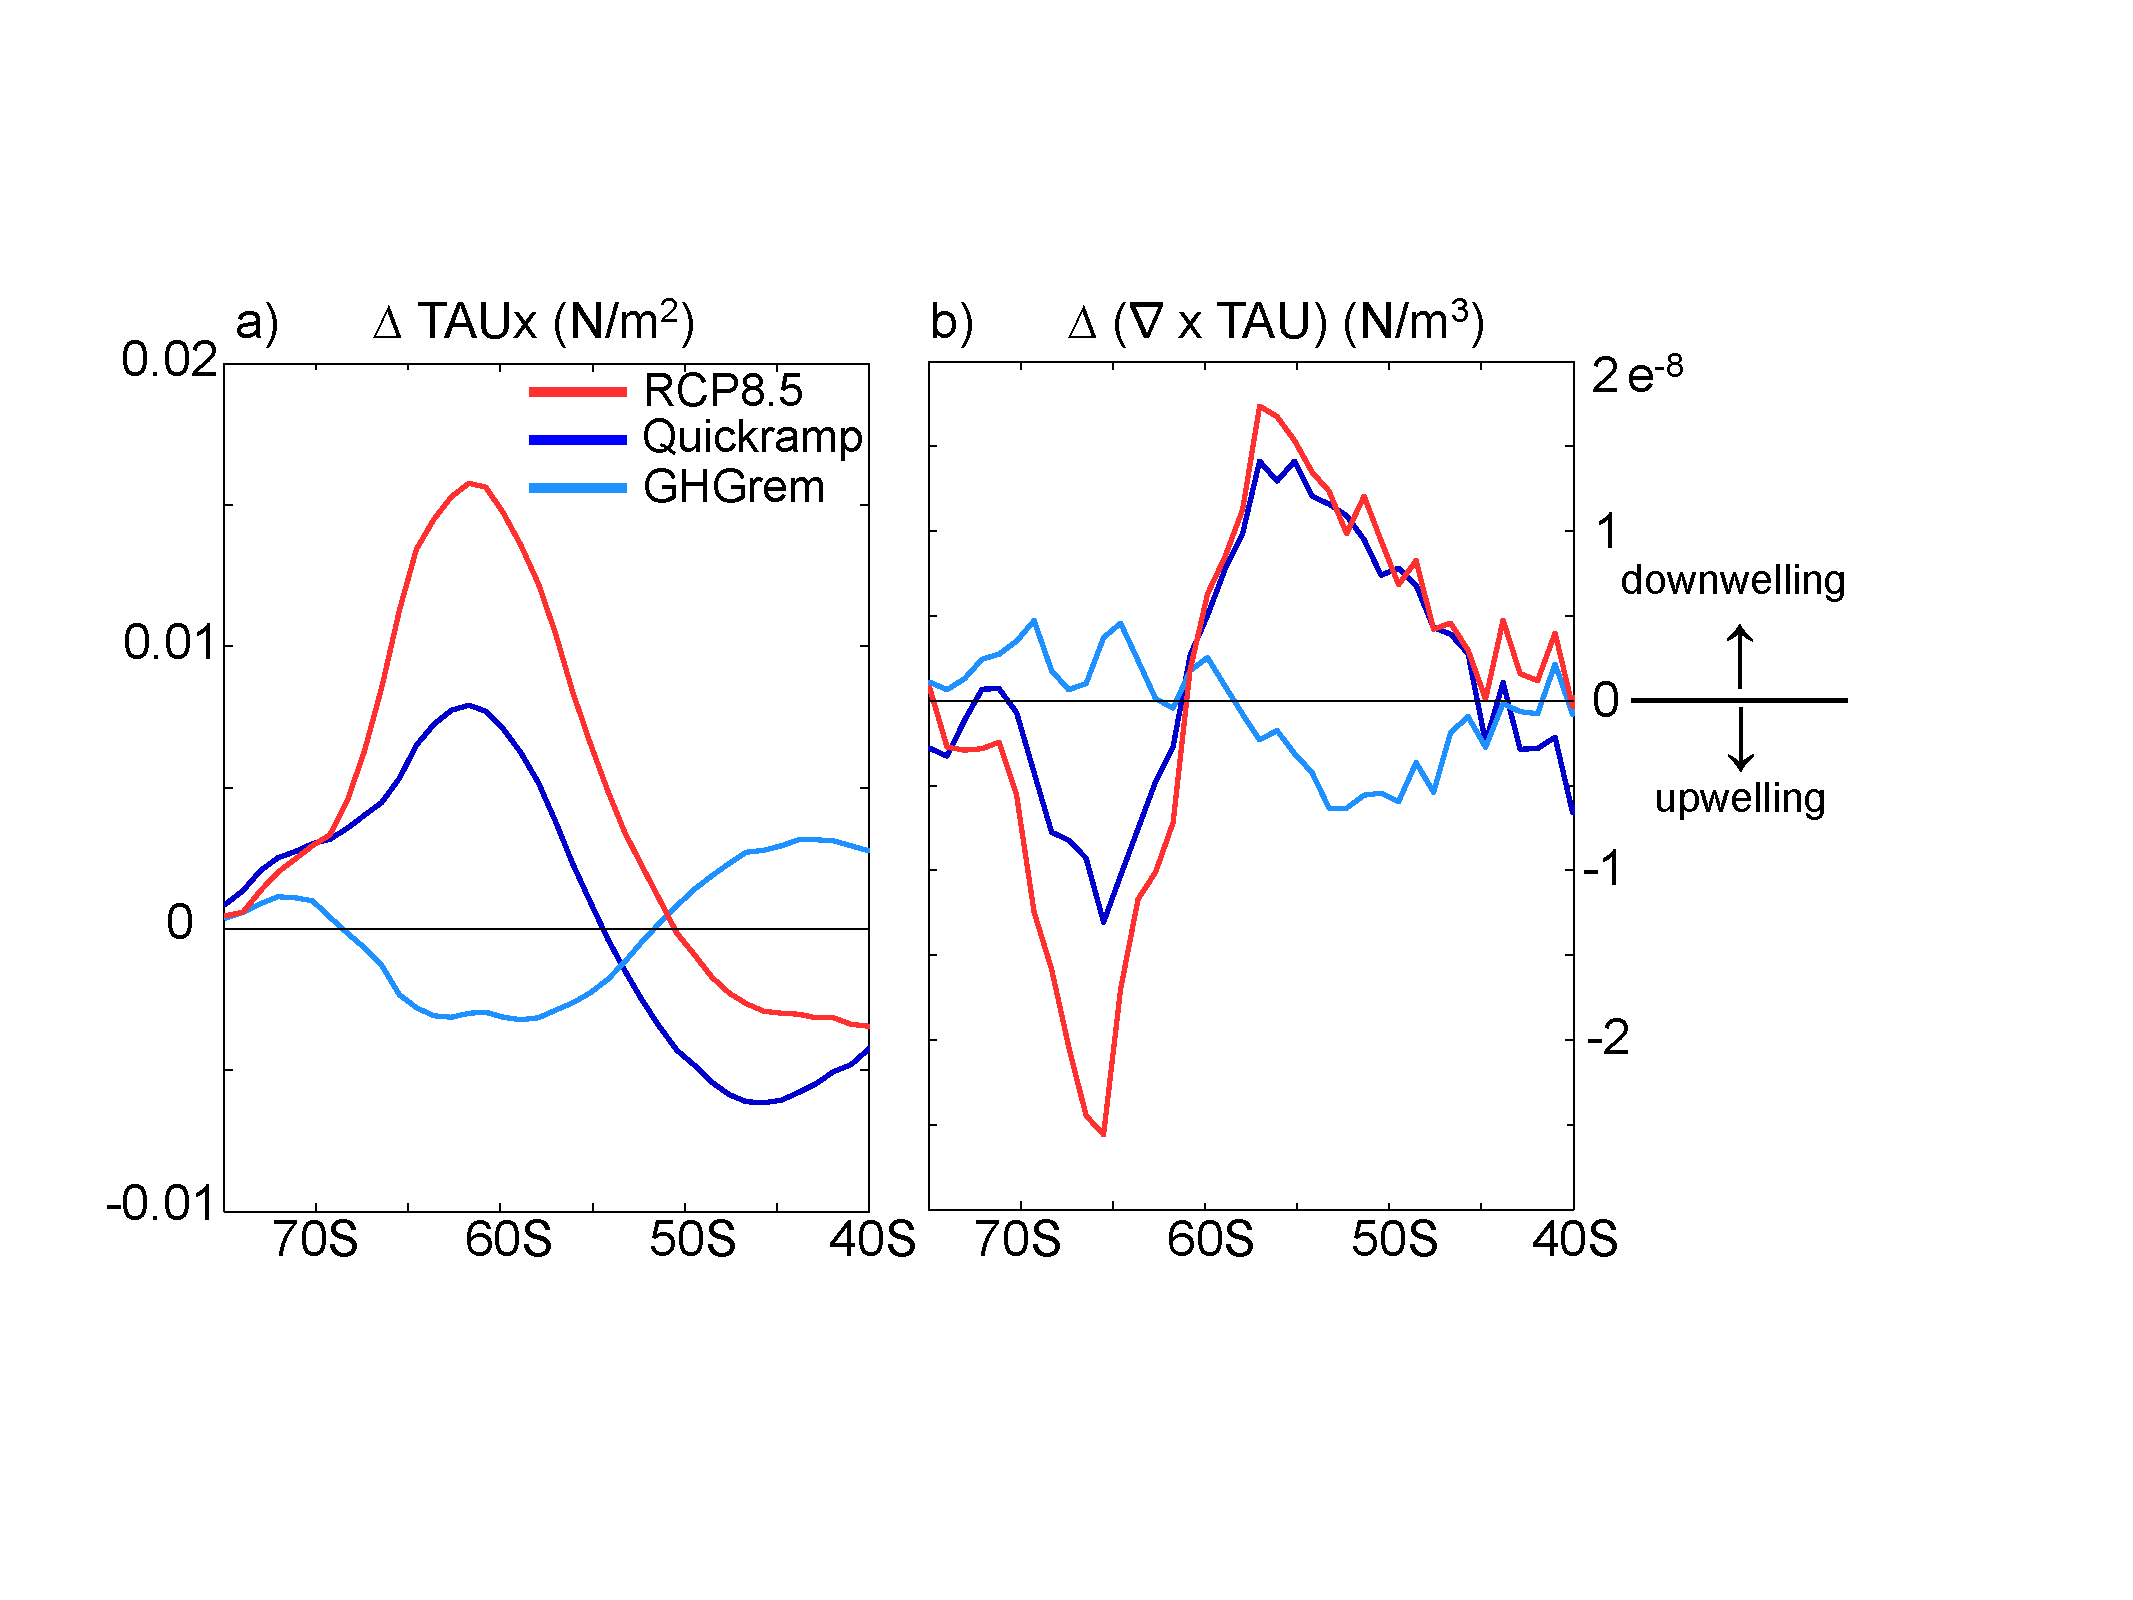
\includegraphics[width=20pc]{figures/zmTAU2.pdf}
%\caption{\textbf{Zonal mean wind stress and wind stress curl anomalies.} Annual mean, zonal mean \textbf{(a)} zonal wind stress (N/m$^2$) and \textbf{(b)} curl of the wind stress (N/m$^3$) over ocean only, as anomalies from 20thC (1970-1999 mean). Positive indicates westerlies in (a) and downwelling in (b).}
%\label{fig:zmtau}
%\end{figure}

% %%%% extra from dissertation
%There are two important factors that contribute to the subsurface temperature anomalies exhibited in Sulf and GHGrem: the ocean heat uptake that occurred prior to the initiation of climate engineering, and the change in wind stress inducing changes in upwelling strength. The ocean heat uptake causes the subsurface ocean waters to be warmer at the start of climate engineering, particularly in the level of the CDW but also deeper throughout the water column (see year 2035 in Figure \ref{fig:quickSOprog} and Figure \ref{fig:ghgremSOprog}), and the wind stress anomalies cause this anomalously warm CDW (which is already warmer than waters above it in the mean state) to be upwelled closer to ice sheet outlets. 

%Examination of the time evolution of temperature anomalies in Sulf (Figure \ref{fig:quickSOprog}) compared to GHGrem (Figure \ref{fig:ghgremSOprog}) suggests that the primary difference in the amount of warming near ice sheets between the two scenarios, however, is likely the upwelling strength. However, further quantification of the mechanisms for the warm waters encroaching on ice shelves (previously warmed water from ocean heat uptake, or increased upwelling) is required to conclusively determine the primary contributor. Specifically, heat contributions from anomalies in circulation acting on the mean temperature gradient ($\textbf{V}' \nabla \bar{T}$) should be compared to those from anomalies in temperature acting on the divergence in the mean circulation field ($T'\nabla\cdot \bar{\textbf{V}}$), which will be a subject of further work. % @@ could also be changes in sfc buoyancy and mixing? 9/2/14
% @@ cite marshall and speer 2011 (SO MOC review) here somewhere? or find original ref from that paper...

% %%%%%
\section{Discussion}

%The opposing features induced by the addition of stratospheric aerosols versus the removal of GHGs highlights the inability of the stratospheric sulfate aerosols to counter greenhouse gas-induced circulation changes and associated feedbacks. In particular, increased ocean temperatures combined with residual Southern Ocean circulation anomalies allow warmer ocean waters to access ice sheet outlet regions, leaving open the possibility of destabilization even when climate engineering is employed. %Furthermore, these Southern Ocean anomalies persist throughout the century in our simulations --- ocean temperatures averaged south of 50$^\circ$S, indicate that residual warmth at all depth until at least 2065 in Sulf, with only the top few hundred meters cooling by 2095 (not shown). In contrast, GHGrem shows immediate surface cooling that continues to deepen until the end of the simulation. These differences are also reflected in surface temperatures and zonal wind stress (not shown) over the Southern Ocean until the end of the century.


%@@add something about increasing CDW due to seasonal wind stress?

%@@talk about how it's not just transient: see time v depth/lat plots.
%@@consider 200-800m temp maps (not as good in the end). also, check SH full zonal climo. Also redo SH maps w/ zoomed in
%@@move on to subsfc ocean: show time v depth plots of just Southern ocean TEMP plus maybe SHF in just the SO? Finale will be zonal means of TEMP with depth and ocean TEMP in 200-500m layer (plus perhaps the sector zonal means).
%@@Need to ref my other 2 papers
% change in wind stress curl zero crossings:
% Quickramp: -0.26268 deg
% GHGrem1850: 0.14516 deg
% RCP8.5: -0.27351 deg

%\begin{figure}[htbp] % the star afterwards makes it a one column fig in a 2-col document
%\centering
% \noindent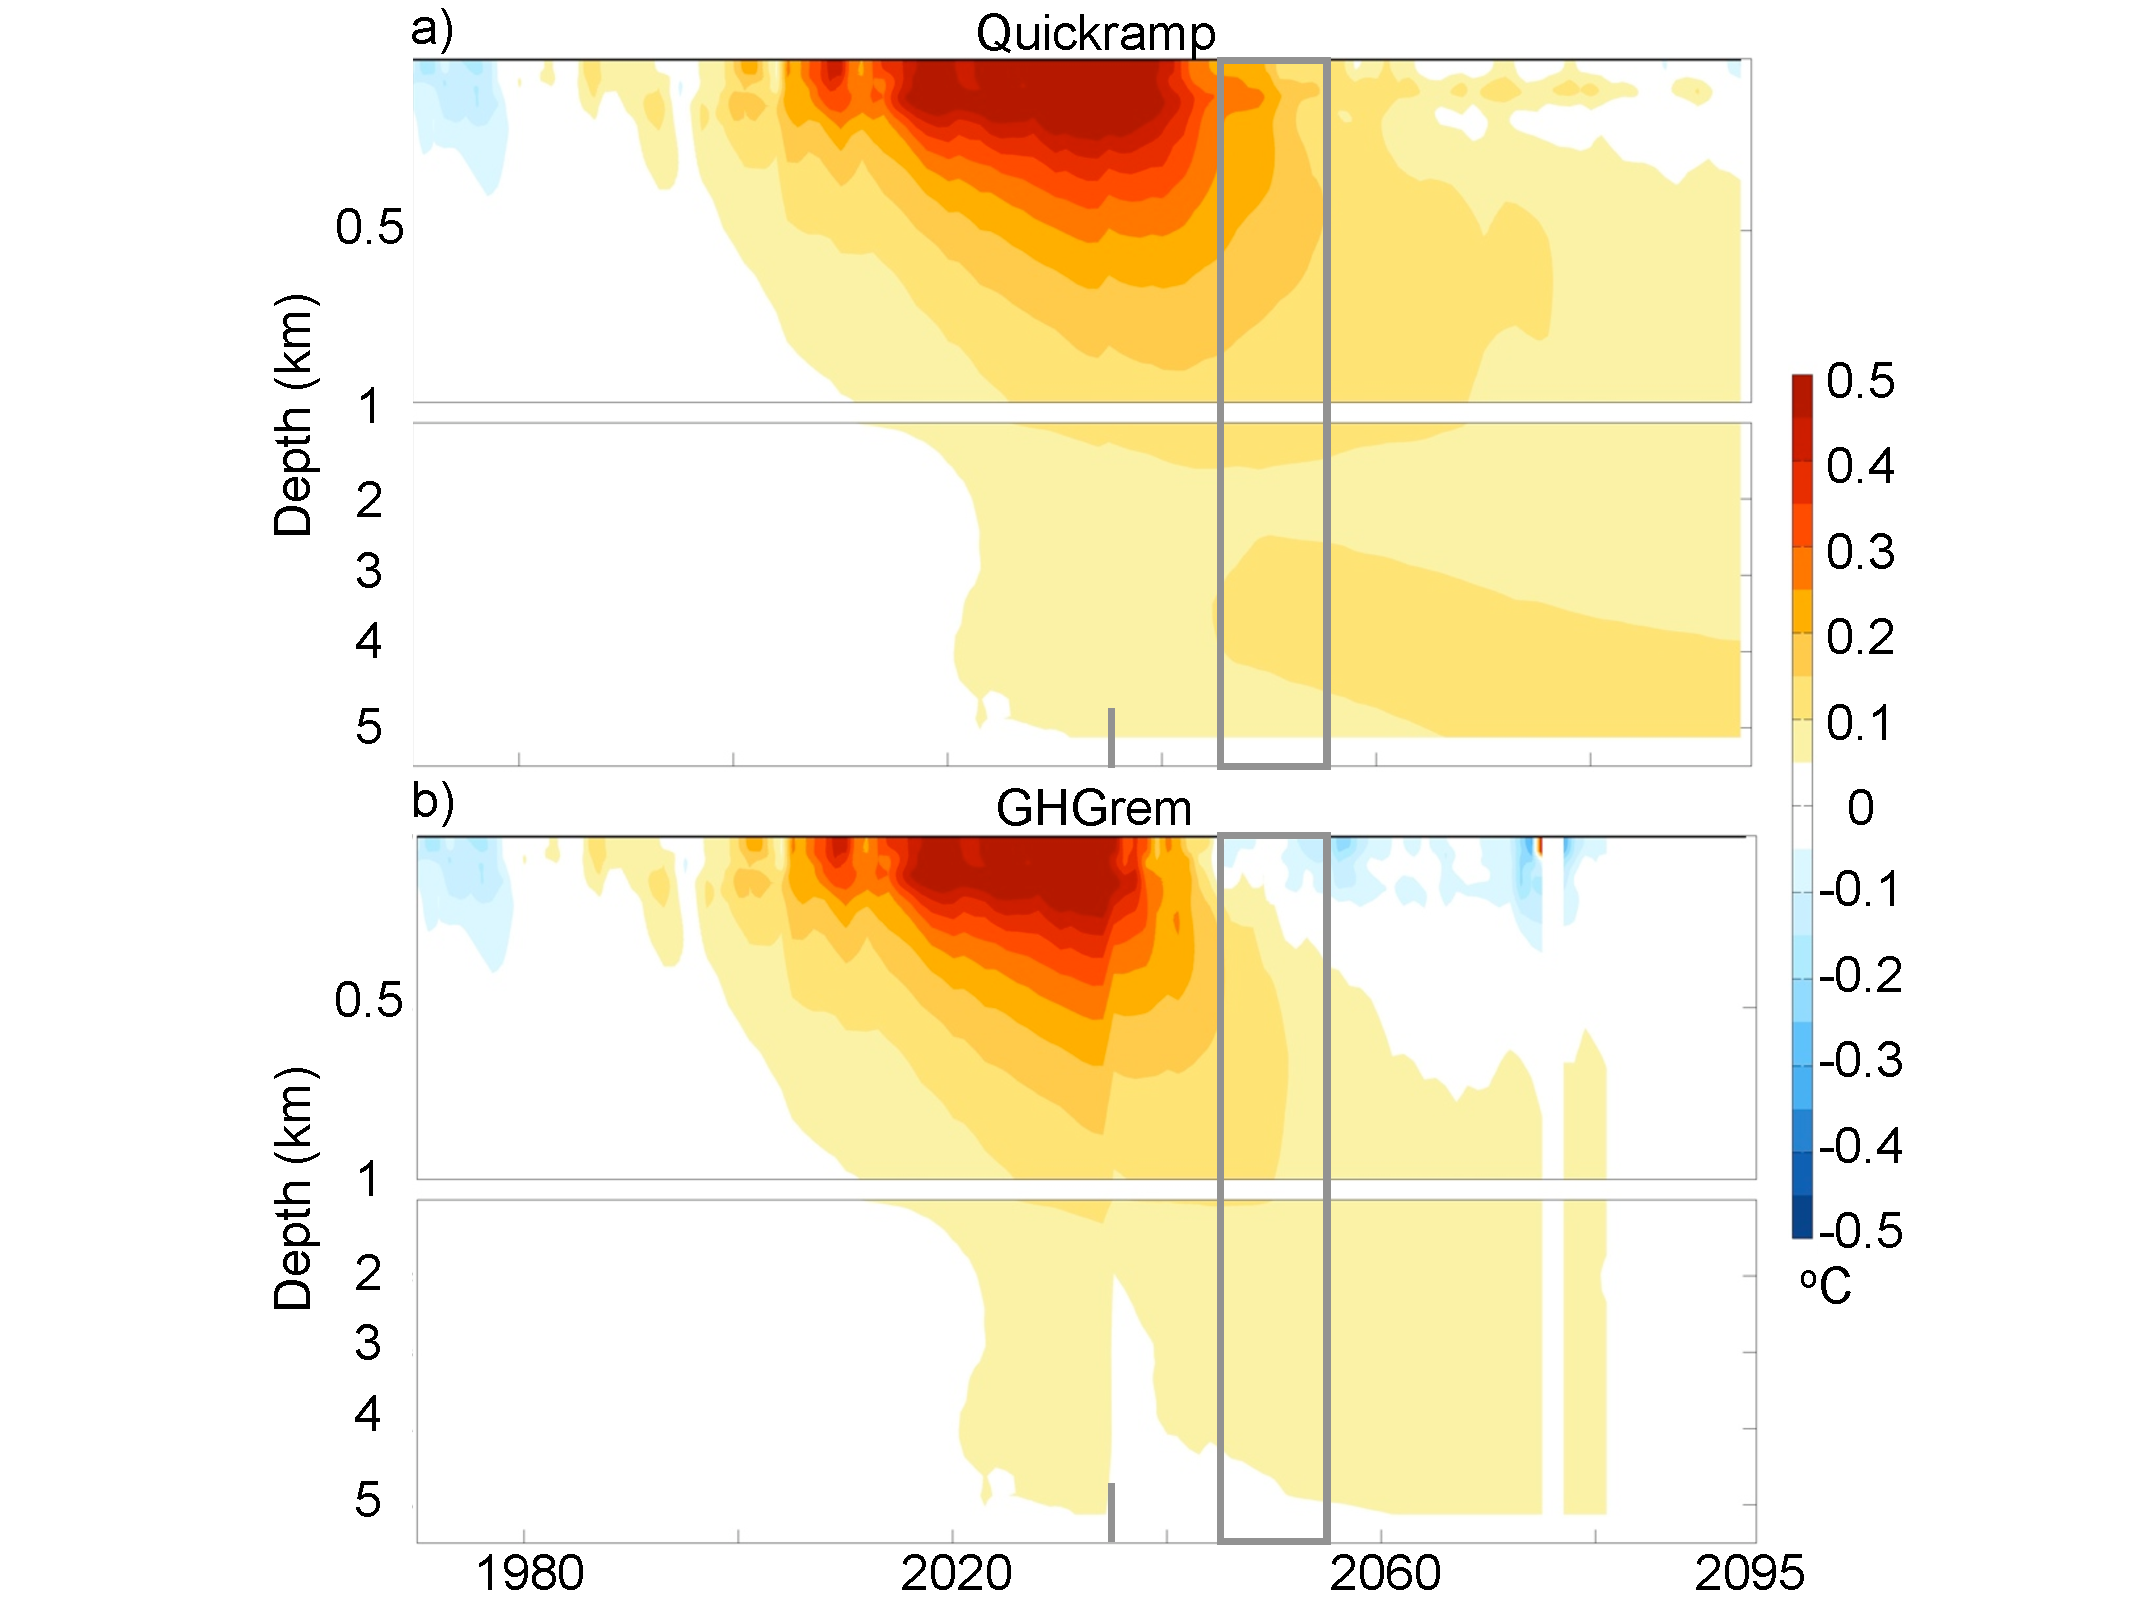
\includegraphics[width=20pc]{figures/SOTEMPtime2.pdf}
%\caption{\textbf{Averaged Southern Ocean temperature anomalies with depth and time.} Annual mean, Southern Ocean mean (south of 50$^\circ$S), zonal mean ocean potential temperature ($^\circ$C) anomaly from 20thC (1970-1999 mean), with depth (km) and time (years). Years 1970-2005 are 20thC anomalies, years 2006-2034 are RCP8.5 anomalies, and years 2035 onward (denoted by the large gray tick mark) are \textbf{(a)} Sulf and \textbf{(b)} GHGrem anomalies. Gray boxes indicate the years of averaging for previous figures, in particular Figures \ref{fig:shsubtemp}e and \ref{fig:shsubtemp}f.}
%\label{fig:sotemptime}
%\end{figure}

%\begin{figure*}%[htbp] % the star afterwards makes it a one column fig in a 2-col document
%\centering
% \noindent\includegraphics[width=39pc]{figures/SHzonmeanTEMP.pdf}
%\caption{Annual mean, zonal mean ocean potential temperature ($^\circ$C) anomaly, with depth (m), from the 20thC (1970-1999 mean) \textbf{(a)} RCP8.5, \textbf{(b)} Quickramp, and \textbf{(d)} GHGrem years 2045-2054. @@Add ocean temp 200-500m @@ Remove RCP8.5 i think. we know that each geo option is "better" than nothing}
%\label{fig:shzmtemp}
%\end{figure*}


% @@ put GHG concentrations fig in "supplementary"?

% answer: s the SAT response pattern indicative of ``delayed Southern Ocean cooling", analogous to the well-known delayed warming, or is this asymmetry unique to sulfate geoengineering? Does the SAT pattern reflect similar subsurface ocean temperature features? And finally, how might this affect Antarctic ice sheet stability?
% @@ other points: tropical SSTs can affect SH circulation in a way that increases warm atmospheric advection to WAIS and forces more CDW into at-risk ice shelve regions
% sea ice generation that produces dense salty water plays a role in getting warm CDW up onto continental shelves (see Joughin11, ocean instability section)
% if get to the point where I include PIG sector figures: jacobs11 and jenkins11 are potentially good refs.
% @@ say more about the first section of the paper: timescales.....
SRM using stratospheric aerosols has been suggested as a `backstop' measure that could be rapidly deployed to avoid so-called climate emergencies, one of which is sea level rise due to destabilization of marine ice sheets \cite{blackstock09}. Here we show that while the rapid addition of stratospheric sulfate aerosols may immediately stop and reverse global mean steric sea level rise at the expense of large land SAT trends, it does not counteract circulation changes that make warmer subsurface waters more available for basal melting of ice shelves around Antarctica. Because these circulation changes are fundamentally due to modification of the stratospheric meridional temperature gradient through the combination of sulfate aerosol deployment and increased GHGs, these circulation changes persist for as long as GHGs and sulfates are in the atmosphere, significantly delaying both surface and subsurface cooling over and in the Southern Ocean (not shown). We also find that, alternatively, reducing greenhouse gases in the atmosphere does counterbalance circulation changes and is hence significantly more effective at cooling the Southern Ocean, and especially the region encompassing Antarctica's largest contributor to sea level rise \cite{shepherd12}: the already unstable Pine Island Glacier outlet \cite{rignot14}. Given that the PIG grounding line is currently retreating along a retrograde bed, its reversibility may only be achievable with significant reductions in basal melt rate past present day rates \cite{favier14} --- a task only removal of GHGs can accomplish based on our results.
%Additionally, % teleconnections
% @@another point: the longer one waits, 1. the more sulfate necessary and 2. the more heat has been buried in the ocean that could reach the ice shelves.
%@@ This result provides yet more evidence for the inadequacy of SRM via stratospheric sulfate aerosols and more evidence for reduction of GHGs as the best method of avoiding climate emergencies.

%The long timescale of response of the ocean also means that 

%One implication of our results is that the more ocean heat uptake that occurs prior to the start of SRM, the greater the risk of warmer waters encroaching on ice shelves even after SRM commences. %These results can be extrapolated to include marine outlet glaciers in Greenland, which SRM has previously been shown via surface mass balance calculations to effectively preserve \citep{irvine09}. However, basal melt is also very important to the health of the Greenland ice sheet, and has been implicated as the cause of the recent acceleration of its outlet glaciers (e.g., \cite{dholland08}). Thus, subsurface ocean conditions must also be considered in evaluating the ability of stratospheric aerosols or SRM in general to preserve the Greenland ice sheet.

We emphasize that surface and subsurface temperatures are undoubtedly cooler when stratospheric aerosols are in use than under business-as-usual warming. However, while general circulation models such as the one we employ do not resolve ice shelves and sub-scale processes that influence their thickness (e.g., small-scale mixing, tidal currents; \cite{joughin11}), we have shown that the large-scale oceanic environment under stratospheric sulfate aerosols after a period of warming would be favorable for further thinning of Antarctic ice shelves, particularly in the at-risk PIG region. Furthermore, the more ocean heat uptake that occurs prior to the start of SRM, the greater the risk of warmer waters encroaching on ice shelves even after SRM commences.

Thus, while the injection of stratospheric aerosols may be effective at avoiding some eventual climate impacts due to global warming, this strategy may not be effective at avoiding one of the oft cited climate ``emergencies": destabilization of the West Antarctic ice sheet. Given the host of potential problems already associated with stratospheric aerosol injections --- including but not limited to ozone depletion \cite{tilmes08,heckendorn09}, risk of extreme regional temperature trends upon cessation (e.g., \cite{mccusker14}), continued ocean acidification \cite{feely04}, and reduced precipitation (e.g., \cite{bala08}) --- our results contribute further evidence as to why a reduction in GHGs is a much more highly desirable solution. % This may especially be the case if the WAIS is observed to already be destabilizing before stratospheric sulfates are deployed. Preemptive deployment might then avoid this risk, however we have also shown that a reduction in greenhouse gases would be more effective at preserving WAIS. 


\begin{methods}

%\section{Methods}

In order to capture the relevant range of climate system timescales and dynamical feedbacks, we use the Community Climate System Model version 4 (CCSM4, \cite{gent11}), a global climate model (GCM) with a finite volume 0.9$^\circ$x1.25$^\circ$ resolution atmosphere coupled to a 1$^\circ$ full-depth ocean, sea-ice, and land models. The full-depth ocean is required in order to obtain a more realistic regional response \cite{mccusker12} and to incorporate the long timescales stemming from heat exchange with the deep ocean. %We simulate two SRM climate engineering scenarios that bookend possible scenarios that could be implemented in the future. 

Two simulations from the National Center for Atmospheric Research (NCAR) are used as controls: the Climate Model Intercomparison Project 5 (CMIP5) ``business-as-usual" scenario, called Representative Concentration Pathway 8.5 (RCP8.5), reaching a radiative forcing from greenhouse gas emissions of 8.5 W/m$^{2}$ above preindustrial levels by 2100, and the 20th century simulation (20thC) forced with historical greenhouse gas and aerosol emissions plus volcanic eruptions. The climate engineering simulations are branched from RCP8.5 at year 2035 when the global mean surface air temperature (SAT) is approximately 1$^\circ$C greater than that of the end of the 20th century average (computed for years 1970-1999). In year 2035, a prescribed stratospheric sulfate aerosol burden (as in \cite{mccusker12} and \cite{mccusker14}) is commenced that is ramped up from zero at a rapid rate of increase. The scenario has 3 years of rapid ramping at 8 teragrams of sulfate (SO$_4$) per year (Tg/yr), followed by ramping at 0.67 Tg/yr for the remainder of the simulation (calculated to provide a roughly equal and opposite radiative forcing to the RCP8.5 scenario transiently). %The Slowramp scenario has 50 years of `slow' ramping at 1.1 Tg/yr. After 50 years, the quick and slow scenarios reach approximately the same sulfate burden, and ramp together at 0.67 Tg/yr for the remainder of the simulations. % The right panel of Figure \ref{fig:tsts} displays the sulfate ramping scenarios.

We conducted an ensemble of four sulfate engineering simulations, initialized from four RCP8.5 ensemble members. Henceforth, we will refer to the ensemble average as Sulf. We contrast the sulfate engineering scenario with an idealized representation of complete mitigation and carbon sequestration by conducting one simulation, called GHGrem, in which greenhouse gases (CO$_2$, CH$_4$, N$_2$O, and CFCs 11 and 12) are abruptly set to year 1850 levels in the year 2035. Unless otherwise noted, anomalies are presented as the departures of the average response (Sulf, GHGrem, and RCP8.5) in years 2045-2054 from the 1970-1999 average from the 20thC simulation.%Epoch means considered in the present analysis are for years 1970-1999 of 20thC and years 2045-2054 of Quickramp, Slowramp, GHGrem, and RCP8.5, unless otherwise noted. %The 'quick' rate of increase amounts to a 2.67 teragrams of sulfur equivalent (TgS) increase per year for the first 3 years, followed by a smaller rate of about 0.28 TgS per year, so that it provides a roughly equal and opposite radiative forcing to the \textit{rcp8.5} scenario transiently until the end of the simulation in year 2095. The 'slow' rate is equal to a constant rate of increase of 0.37 TgS per year for 50 years, followed by 10 years of the same rate as quickramp, 0.28 TgS.  %@@Add something about how these amounts compare to Pinatubo. @@ Need to update figs w/ slowramp to have ensemble data.

\end{methods}

%% Put the bibliography here, most people will use BiBTeX in
%% which case the environment below should be replaced with
%% the \bibliography{} command.

%\begin{thebibliography}{1}

%\end{thebibliography}


%\bibliographystyle{ametsoc}
\bibliography{allrefs}
% ~/bibtexrefs/allrefs  == this is version controlled now, but will have to just copy into current dir?


%% Here is the endmatter stuff: Supplementary Info, etc.
%% Use \item's to separate, default label is "Acknowledgements"

\begin{addendum}
\item[Acknowledgements] This research was funded by the Tamaki Foundation and supported in part by the Na- tional Science Foundation through TeraGrid resources provided by the Texas Advanced Computing Center under Grant TG-ATM090059.
\item[Author Contributions] 
 \item[Competing Interests] The authors declare that they have no competing financial interests.
\item[Correspondence] Correspondence and requests for materials should be addressed to K.E.M.~(email: kemccusk@uvic.ca).
\end{addendum}

%%
%% TABLES
%%
%% If there are any tables, put them here.
%%

\end{document}
